% !TEX TS-program = pdflatex
% !BIB TS-program = bibtex8
\documentclass{ccjnl}

\usepackage{array}
\usepackage{booktabs}
\usepackage{float}
\usepackage{placeins}
\usepackage{graphicx}
\usepackage{subfig}
\usepackage{multirow}
\usepackage{listings}
\usepackage{xcolor}
\usepackage{amsmath}
\usepackage{caption}
\usepackage{enumitem}
\usepackage{needspace}
\usepackage{makecell}




% Compact and non-stretchable float spacing






\lstset{
	basicstyle=\ttfamily\scriptsize,
	breaklines=true,
	frame=single,
	columns=fullflexible,
	keepspaces=true,
	xleftmargin=0pt,
	xrightmargin=0pt
}

\ccjnlset{
  classification={EMERGING TECHNOLOGIES \& APPLICATIONS},
  doi={10.23919/JCC.fa.2026-0311.202609},
  volume={23},
  issue={9},
  publication-year={2026},
  first-page={341},
	title          = {Internet of Compute: Fundamentals, Architecture, Key Technologies, and Scenario Experiments},
	cite-title     = {Internet of Compute: Fundamentals, architecture, key technologies, and scenario experiments},
	corr-email     = {liweibupt@bupt.edu.cn},   
}

\author*[addr1,addr2]{Wei Li}[style=chinese]
\author[addr2]{Weibo Zhao}[style=chinese]
\author[addr2]{Runyan Wang}[style=chinese]
\author[addr2]{Liu Sang}[style=chinese]
\author[addr2]{Jinfei Huang}[style=chinese]
\author[addr1]{Songlin Sun}[style=chinese]
\author[addr2]{Ruming Liu}[style=chinese]
\author[addr2]{Yue Su}[style=chinese]
\author[addr2]{Fei Ma}[style=chinese]

\address[addr1]{Beijing University of Posts and Telecommunications, Beijing 100\,876, China}
\address[addr2]{China Academy of Information and Communications Technology, Beijing 100\,191, China}

\begin{document}
	\maketitle
\enlargethispage{-2\baselineskip}

\begin{abstract}
Traditional Internet architectures struggle to perceive and schedule computing resources, while existing Compute and Network solutions suffer from closed control planes and inefficient transmission protocols. To address these limitations, we propose the Internet of Compute (IoC), a next-generation network architecture supporting cross-domain intelligent task scheduling. We introduce “resource state entropy” and a network capacity model as the theoretical foundation to quantify the dynamics and equilibrium of computing, network, and storage resources. Based on entropy balance, we construct a novel three-tier architecture featuring an independent Interconnection Resource Layer. Furthermore, we propose the Computing Resource Identifier (CRID) for unified resource positioning, the Resource-Defined Memory Access Protocol (RDMAP) for long-distance lossless transmission, and an entropy-balance scheduling algorithm for global resource matching. Experimental results in large language model(LLM) training and inference scenarios demonstrate that our approach significantly improves resource matching accuracy and cross-domain transmission efficiency, validating the feasibility of the IoC architecture.
\keywords{Internet of Compute (IoC); Computing Resource Identifier (CRID); entropy balance; Resource-Defined Memory Access Protocol (RDMAP); resource state entropy}
\end{abstract}

\section{Introduction}
\label{s1}
With the rapid development of technologies such as artificial intelligence (AI), big data, and edge computing, traditional Internet architectures are increasingly revealing limitations in supporting large-scale, low-latency, and high-reliability compute scheduling. Although the classic TCP/IP system successfully achieved global general-purpose data transmission, its design paradigm of decoupling the bearer network from the service network~\cite{1}, with no separation of the control plane and data plane~\cite{2} makes it difficult to effectively perceive and schedule upper-layer computing resources~\cite{3,4,30}. In recent years, computing demand has evolved from centralized cloud data centers~\cite{5} to a ubiquitous cloud-edge-terminal distribution~\cite{6}, necessitating a new generation of network architecture~\cite{7} capable of deep integration across computing, storage, and networking~\cite{8}.

In this context, the Internet of Compute (IoC) emerged. This concept was first proposed by the China Academy of Information and Communications Technology (CAICT) in 2025~\cite{9}, aiming to build a next-generation architecture that supports intelligent scheduling of computing tasks across domains, subjects, and levels. Its core goal is to break the barriers between existing networks and computing resources through unified identification~\cite{10}, programmable protocols~\cite{31}, and collaborative scheduling mechanisms, achieving internet-level interconnection and efficient utilization of computing resources. Based on previous work, this paper systematically expands the theoretical foundation of the IoC, proposes a unified architecture integrating the ternary relationship of computing, storage, and networking, and makes key technical breakthroughs in protocol design, resource identification, and scheduling algorithms.

The specific research content of this paper is summarized below.
\begin{itemize}[nosep]
	\item Theoretical Expansion: Improving the concept of the IoC to fully cover the relationship between computing, storage, and networking, and adding theories such as “network resource state entropy” and “network capacity models”.
	\item Architectural Updates: Constructing a new Interconnection Resource Layer based on the principle of resource state entropy balance, including transport control protocols and Computing Resource Identifier (CRID).
	\item Technical Innovation: Proposing the Resource-Defined Memory Access Protocol (RDMAP) for long-distance lossless transmission and novel scheduling algorithms based on CRID.
	\item Scenario Use Cases: Defining architectures and key technologies for two major scenarios: large language model(LLM) training and inference.
	\item Experimental Verification: Conducting experiments on CRID, RDMAP, and scheduling algorithms in AI training and inference scenarios.
\end{itemize}

\section{Related Work}
\label{s2}

\subsection{Evolution of Network Architecture}
\label{s2-1}
The Internet originated from the idea of packet switching in the 1960s, and the establishment of the TCP/IP protocol suite in the 1970s laid the foundation for its core feature of open interconnection. This system adopts a five-layer protocol stack, with the service network decoupled from the bearer network. The bearer network only provides general transmission capabilities, is unaware of upper-layer applications, and has not yet separated the control plane from the forwarding plane~\cite{11}.

Subsequently, distributed computing emerged, mainly represented by grid computing and cloud computing. Grid computing focuses on cross-organizational collaboration of compute~\cite{12,13}, while cloud computing emphasizes the pooling~\cite{14} and on-demand delivery~\cite{15} of IT resources~\cite{16}. Although cloud-edge collaboration and cloud services deeply integrate network capabilities at the commercial level, this integration remains superficial. The deep, native integration of computing and networking has not been realized at the protocol stack and scheduling mechanism levels, leading to persistent matching gaps between task demands and resource provisioning. 

In recent years, paradigms such as Compute Network, Converged Computing and Networking, Computing-First Network, and Computing-Aware Network (CAN) have attempted to integrate heterogeneous compute from the network side~\cite{28}. However, these existing solutions are fundamentally transport-centric extensions rather than architectural reinventions. They treat computing as terminal nodes attached to the network, relying on heuristic routing and tightly coupled, closed control planes. This closed nature makes it difficult to support flexible cross-subject and cross-regional compute scheduling. Meanwhile, the lack of low-latency~\cite{17} programmable transmission protocols~\cite{19} prevents the Internet-scale wide interconnection of compute resources~\cite{20} as an open resource pool.

NVIDIA put forward the vision of a global network of GPU compute. Through high-speed interconnection, a unified software stack, and cloud-edge-end collaboration, it integrates GPU resources distributed in global data centers, edge nodes, and end devices into a logically unified supercomputing platform. While this reflects the evolutionary trend of ubiquitous compute, it remains a vendor-specific, hardware-centric solution rather than an open, fundamental network architecture evolution.


\subsection{Related Research on the IoC}
\label{s2-2}
To bridge the aforementioned gaps, the IoC was proposed as a next-generation architecture for interconnecting geographically distributed compute resources~\cite{9}. Unlike CAN or Resource-Aware Networks, which primarily focus on steering traffic to available compute, IoC introduces a fundamental conceptual breakthrough: treating the “computing task” as the primary scheduling entity, akin to data packets in the traditional Internet.

IoC aims to build a next-generation network architecture that supports cross-domain scheduling of computing tasks. Its core innovation lies in introducing a unified CRID and protocol interface to enhance the interconnection of heterogeneous compute~\cite{18} and high-performance cross-domain transmission. By decoupling the control plane from the bearer network, IoC forms an independent logical interconnection resource layer. This architectural shift transforms the scheduling paradigm from network-driven traffic routing to task-driven resource matching, breaking through the limitations of existing paradigms in cross-subject scheduling and wide-area collaboration.

\section{Fundamental Theories of the IoC}
\label{s3}
Building upon previous architectural research, this paper systematically proposes a fundamental theoretical system for the IoC. To address the lack of algorithmic breakthroughs in distributed resource abstraction and scheduling, this theoretical system is anchored by the concept of Entropy Balance. It provides a mathematically quantifiable framework that fully covers task demand modeling, dynamic compute-network-storage resource capacity evaluation, and cross-domain collaborative scheduling mechanisms.

\subsection{Definition of the IoC}
\label{s3-1}
The IoC is an enhanced evolutionary form of the Internet oriented toward computing tasks. It fundamentally shifts the operational logic from “host-to-host data transmission” to “task-to-resource matching.” By constructing a unified CRID and protocol interface, IoC strengthens heterogeneous compute and cross-doma-performance transmission capabilities. This enables computing tasks and their associated data to be accurately matched with adaptive resources, thus forming a logically interconnected network with intelligent perception, real-time discovery, and on-demand acquisition capabilities.

The interconnected objects cover IT software and hardware resources such as computing, storage, and networking. The service objects are task-based applications, which are characterized by clear start–end boundaries, bursty and diverse resource demands—such as AI Inference, AI training, and video rendering.

\subsection{Demand Characteristics of Task-Based Applications}
\label{s3-2}
Different from persistent online services, task-based applications feature explicit input and output, resource release upon completion, strong demand burstiness, obvious periodicity, and high diversity, relying heavily on computing–network collaboration.

Based on resource demand attributes, application forms, and deployment constraints, the fundamental theory of IoC must satisfy four core characteristics to distinguish itself from traditional heuristic-based resource allocation:
\begin{itemize}[nosep]
	\item Elasticity
	
	Networks and compute shall dynamically adapt to task characteristics. In response to the discreteness of AI tasks, the system should schedule tasks and data flows on demand, and seamlessly expand to remote resources when local compute is insufficient. This breaks the siloed mode of rigid transmission in traditional networks and the isolated deployment of compute in cloud-edge paradigms, fully exploiting the lossless transmission capability of Remote Direct Memory Access (RDMA).
	\item Predictable Capacity
	
	Traditional information entropy only optimizes information coding and cannot characterize the randomness of task–resource matching in dynamic computing networks. As an algorithmic breakthrough, this paper extends entropy theory to the compute dimension and proposes models of compute state entropy and network transmission entropy. The former quantifies task arrival rate and resource demand fluctuation, while the latter describes bandwidth utilization and delay jitter.
	
	The mathematical coordination of the two enables accurate, proactive prediction of compute pools and network bandwidth. For instance, when batch training requires multiple GPUs, the system identifies the local shortage in advance via entropy evaluation, triggers cross-domain invocation, and synchronously reserves a corresponding link. This fundamentally solves the problems of blind compute supply and idle network resources prevalent in existing resource-aware networks.
	
	\item Resource Pooling
	
	Faced with the fragmentation of heterogeneous resources (CPU, GPU, TPU, etc.) caused by geographical and architectural differences, resource pooling abstracts distributed resources into feature vectors of computing, storage, and networking through unified identification. Unlike traditional distributed computing abstractions, IoC characterizes their dynamic states with the aforementioned entropy values, achieving unified management and reuse under a global logical view.
	\item Entropy Balance
	
	
	In response to task diversity and resource heterogeneity, entropy balance serves as the core algorithmic mechanism that distinguishes IoC from traditional load balancing. It does not pursue absolute uniformity of node utilization, but seeks the optimal mathematical trade-off among system performance, resource efficiency, and quality of service.
	
	For example, delay-sensitive inference tasks are preferentially assigned to low-latency, high-computing-performance nodes even if their loads are relatively high; throughput-prioritized training tasks are scheduled to lightly loaded clusters to maximize overall throughput. Its core principle is to match resources to tasks on demand based on quantified entropy states, thereby avoiding local congestion or idleness—a limitation that heuristic-based cloud-edge collaboration fails to overcome.
\end{itemize}

\subsection{Computing Task Model}
\label{s3-3}
This paper models computing tasks using two independent random variables: the number of task arrivals per unit time follows a Poisson distribution with parameter $\lambda$; the service time of a single task follows a normal distribution $T_s\sim\mathcal{N}(\mu,\sigma^2)$, where $\mu$ is the mean service time and $\sigma^2$ is the variance of the service time. Since service time is non-negative, negative samples generated from the normal distribution are discarded and regenerated. Three typical task types are accordingly classified: AI training: low $\lambda$, high $\mu$, belonging to long-duration and low-frequency tasks; AI inference: high $\lambda$, low $\mu$, belonging to short-duration and high-frequency tasks; Video rendering: intermediate characteristics with balanced performance.

This model provides a statistical foundation for resource state modeling and scheduling strategy design. Its characteristic probability distributions are shown in Figure~\ref{fig:Probability Distribution Characteristics}.

\begin{figure}[!ht]
	\centering
	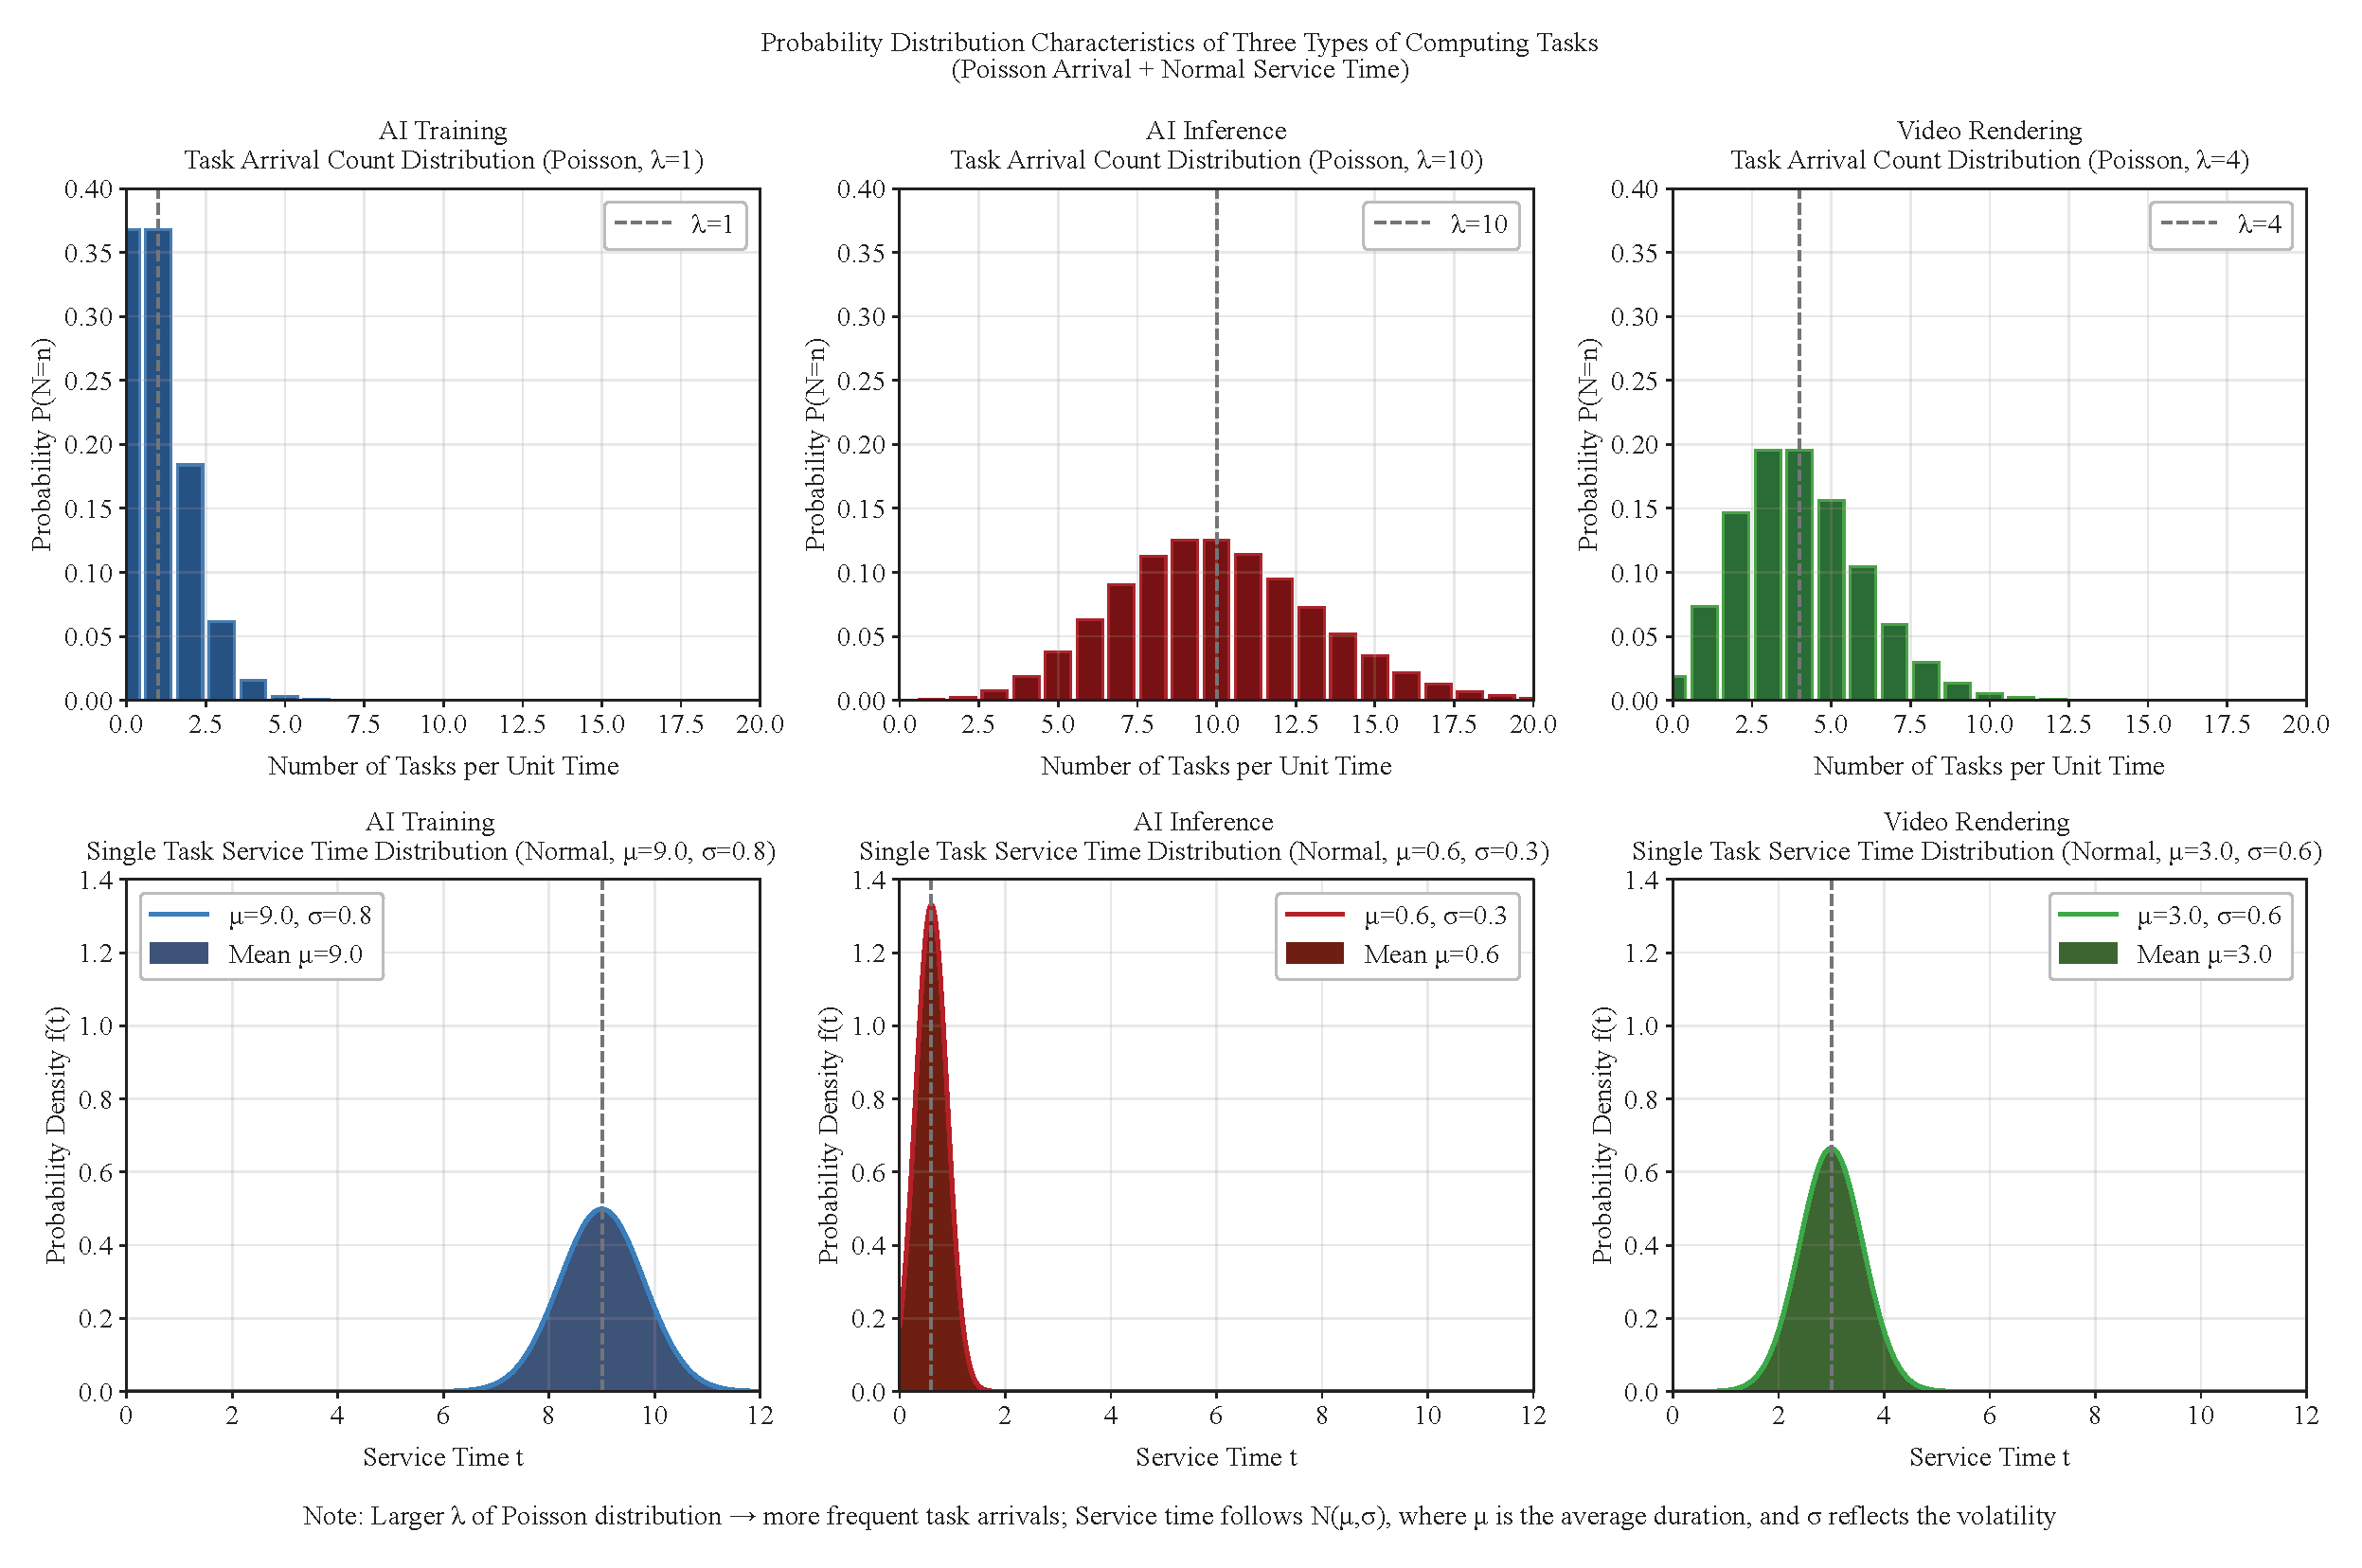
\includegraphics[width=0.90\columnwidth]{figures/figure1.eps}
	\caption{Probability distribution characteristics of three types of computing tasks.}
	\label{fig:Probability Distribution Characteristics}
\end{figure}

\subsection{Resource State Entropy: Quantification of Dynamics and Equilibrium}
\label{s3-4}

On the basis of the previous Computing Resource State Entropy, this paper further introduces Network State Entropy and Storage State Entropy, so as to construct a full-dimensional Resource State Entropy system.

Assume that the whole network contains multiple resource nodes, and the state of each node is composed of a feature vector including computing utilization, network utilization, and storage utilization. Resource State Entropy is defined as a measure of the uncertainty of a node’s state: the more stable the state, the lower the entropy; the greater the fluctuation, the higher the entropy.

Let the network-wide resource matrix be $\mathbf{R}$, which contains $N$ resource nodes, with each resource pool denoted as $\mathbf{r}_i$. The computing resource feature vector is defined as $\mathbf{r}_i(c_i,l_i,s_i)$, where $c_i$ is the available computing state, $l_i$ is the available network state, and $s_i$ is the available storage state, for $i = 1,2,\dots,N$. This paper proposes the concept of “resource state entropy”: for the state of a node $\mathbf{r}_i$, the more stable the state, the lower the entropy; conversely, the more unstable the state, the higher the entropy.

Now define the computing utilization of resource pool $i$ at the $k$-th hour of a day as $c_{ik}$, where $k = 1,2,\dots,24$.

Let $P(c_{ik})$ be the probability that the average utilization appears at each hour of the day.

According to the definition of the entropy function~\cite{22}, we have:

The “computing resource state entropy” of node $c_{ik}$ is
\begin{equation}
	H(c_i) = -\sum_{k=1}^{24} P(c_{ik}) \log\left(P(c_{ik})\right).
\end{equation}

Similarly, let the link bandwidth utilization of the node at the $k$-th moment be $l_{ik}$ with probability $P(l_{ik})$, and the storage occupancy rate at the $k$-th moment be $s_{ik}$ with probability $P(s_{ik})$. We can obtain:

The “network resource state entropy” of the node is
\begin{equation}
H(l_i) = -\sum_{k=1}^{24} P(l_{ik}) \log\left(P(l_{ik})\right).
\end{equation}

The “storage resource state entropy” of the node is
\begin{equation}
H(s_i) = -\sum_{k=1}^{24} P(s_{ik}) \log\left(P(s_{ik})\right).
\end{equation}

Therefore, the resource state of a node can be represented as an entropy vector
\begin{equation}
\mathbf{H}_i = \left(H(c_i), H(l_i), H(s_i)\right).
\end{equation}

\subsubsection{State Types and State Entropy}
\label{s3-4-1}

\begingroup

To characterize dynamic resource usage in the IoC, this paper models node states along two complementary dimensions: node type and utilization interval. Node type reflects the service and load characteristics of hosted tasks, while utilization intervals discretize continuous resource measurements for entropy calculation. In this paper, the logarithm is taken to base 2, and the resulting entropy is measured in bits. The probability of each state is defined as the empirical probability of the corresponding utilization interval, i.e., the proportion of observations falling into that interval over the observation period.

Directly using instantaneous utilization values would generate an excessively large number of states and reduce model generalizability. Therefore, resource
utilization is divided into four representative intervals:
$[0,30\%]$, $[30\%,60\%]$, $[60\%,80\%]$, and $[80\%,100\%]$,
corresponding to idle, low-load, medium-load, and high-load states,
respectively. Table~\ref{tab:computing-resource-entropy} summarizes
the resulting computing-resource entropy distribution.

% Reusable four-row state block for Tables 1--3
\newcommand{\EntropyGroup}[6]{%
	\multirow{4}{2.30cm}{\centering #1}
	& [80\%, 100\%] & #2 & \multirow{4}{*}{#6} \\
	\cmidrule(lr){2-3}
	& [60\%, 80\%] & #3 & \\
	\cmidrule(lr){2-3}
	& [30\%, 60\%] & #4 & \\
	\cmidrule(lr){2-3}
	& [0, 30\%] & #5 & \\
}

% Table 1: computing-resource state entropy
\begin{table}[!t]
	\centering
	\scriptsize
	\setlength{\tabcolsep}{2.7pt}
	\renewcommand{\arraystretch}{1.05}


	\caption{State entropy of computing resources.}
	\label{tab:computing-resource-entropy}
	
	\begin{tabular}{@{}
			>{\centering\arraybackslash}p{2.30cm}
			>{\centering\arraybackslash}p{1.50cm}
			>{\centering\arraybackslash}p{1.35cm}
			>{\centering\arraybackslash}p{1.00cm}
			@{}}
		
		\toprule
		\textbf{State Type}
		& \textbf{\shortstack{Utilization\\Rate}}
		& \textbf{Probability}
		& \textbf{\shortstack{State\\Entropy}} \\
		\midrule
		
		\EntropyGroup{
			A (Inference-intensive, on-demand resource release)
		}{70\%}{20\%}{10\%}{0\%}{1.1568}
		
		\midrule
		
		\EntropyGroup{
			B (Training-intensive, long duration, low arrival rate)
		}{90\%}{0\%}{10\%}{0\%}{0.469}
		
		\midrule
		
		\EntropyGroup{
			C (Rendering, cloud desktops and other relevant workloads)
		}{50\%}{0\%}{50\%}{0\%}{1}
		
		\midrule
		
		\EntropyGroup{
			D (Idle)
		}{0\%}{0\%}{0\%}{100\%}{0}
		
		\bottomrule
	\end{tabular}
\end{table}

Based on their task characteristics and resource usage patterns, four
representative node types are defined as follows.

Type A represents Inference-intensive nodes with short task cycles, light loads, transient resource usage, and elastic compute release. Their network traffic consists of short periods of high bandwidth and frequent establishment and termination of short connections. Storage access is dominated by random reads of small data blocks, particularly model weights, with few writes and concentrated hot spots that are well suited to caching.

Type B represents large-model training nodes with large task scales,
long execution durations, and stable compute occupancy. Such nodes
require persistent, high-bandwidth, and low-jitter connections for
frequent gradient synchronization and parameter exchange, typically
supported by high-performance protocols such as RDMA.

Type C represents real-time interactive workloads, including
rendering, gaming, and cloud PCs. These workloads are GPU-intensive,
highly concurrent, and latency-sensitive, requiring bidirectional,
low-latency streaming transmission. Their storage follows a hybrid
read--write pattern and requires sufficient capacity for resource
preloading and real-time data writes.

Type D represents idle or low-utilization nodes that serve as elastic
resource reserves for bursty task arrivals and global scheduling
balance.

These node types are representative abstractions rather than an
exhaustive classification of business workloads. In practical
deployments, a node may host mixed workloads and transition among
different states over time; such variations are precisely the dynamic
characteristics that resource state entropy is intended to quantify.


% Table 2: network-resource state entropy
\begin{table}[!t]
	\centering
	\scriptsize
	\setlength{\tabcolsep}{2.7pt}
	\renewcommand{\arraystretch}{1.05}
	
	
	\caption{State entropy of network resources.}
	\label{tab:network-resource-entropy}
	
	\begin{tabular}{@{}
			>{\centering\arraybackslash}p{2.30cm}
			>{\centering\arraybackslash}p{1.50cm}
			>{\centering\arraybackslash}p{1.35cm}
			>{\centering\arraybackslash}p{1.00cm}
			@{}}
		
		\toprule
		\textbf{State Type}
		& \textbf{\shortstack{Bandwidth\\Utilization\\Rate}}
		& \textbf{Probability}
		& \textbf{\shortstack{State\\Entropy}} \\
		\midrule
		
		\EntropyGroup{
			A (Inference-intensive, on-demand resource release)
		}{10\%}{10\%}{80\%}{0\%}{0.922}
		
		\midrule
		
		\EntropyGroup{
			B (Training-intensive, long duration, low arrival rate)
		}{90\%}{0\%}{10\%}{0\%}{0.469}
		
		\midrule
		
		\EntropyGroup{
			C (Rendering, cloud desktops and other relevant workloads)
		}{30\%}{40\%}{30\%}{0\%}{1.571}
		
		\midrule
		
		\EntropyGroup{
			D (Idle)
		}{0\%}{0\%}{0\%}{100\%}{0}
		
		\bottomrule
	\end{tabular}
	\par\vspace{8pt}
	% Table 3: storage-resource state entropy
	\centering
	\scriptsize
	\setlength{\tabcolsep}{2.7pt}
	\renewcommand{\arraystretch}{1.05}
	
	
	\caption{State entropy of storage resources.}
	\label{tab:storage-resource-entropy}
	
	\begin{tabular}{@{}
			>{\centering\arraybackslash}p{2.30cm}
			>{\centering\arraybackslash}p{1.50cm}
			>{\centering\arraybackslash}p{1.35cm}
			>{\centering\arraybackslash}p{1.00cm}
			@{}}
		
		\toprule
		\textbf{State Type}
		& \textbf{\shortstack{Storage\\Utilization\\Rate}}
		& \textbf{Probability}
		& \textbf{\shortstack{State\\Entropy}} \\
		\midrule
		
		\EntropyGroup{
			A (Inference-intensive, on-demand resource release)
		}{0\%}{0\%}{50\%}{50\%}{1}
		
		\midrule
		
		\EntropyGroup{
			B (Training-intensive, long duration, low arrival rate)
		}{0\%}{100\%}{0\%}{0\%}{0}
		
		\midrule
		
		\EntropyGroup{
			C (Rendering, cloud desktops and other relevant workloads)
		}{60\%}{20\%}{20\%}{0\%}{1.371}
		
		\midrule
		
		\EntropyGroup{
			D (Idle)
		}{0\%}{0\%}{0\%}{100\%}{0}
		
		\bottomrule
	\end{tabular}
\end{table}


The corresponding state-entropy distributions of network and storage
resources are summarized in
Tables~\ref{tab:network-resource-entropy} and
\ref{tab:storage-resource-entropy}, respectively.

Combining the four representative node types with the four utilization intervals yields fine-grained resource-state combinations that support subsequent entropy calculation and scheduling decisions. Additional node types may be introduced according to deployment environments, business characteristics, and task requirements. Future work will further refine and validate the classification using measured resource data and practical scheduling results.

\endgroup

\subsubsection{Global Entropy of States and Balanced Entropy}
\label{s3-4-2}

It can be seen from Table~\ref{tab:computing-resource-entropy} that node resources are generally in a mixed state of Type~A, Type~B, Type~C, and Type~D, thus being in a state of entropy instability. For a complete resource node $\mathbf{r}_i$, the comprehensive state entropy can be constructed as follows:
\begin{equation}
	H(\mathbf{r}_i) = w_c H(c_i) + w_l H(l_i) + w_s H(s_i),
	\label{eq:comprehensive_entropy}
\end{equation}
where $w_c$, $w_l$, and $w_s$ represent the weights of computing, network, and storage in resources, respectively, reflecting the degree of influence of each type of resource on service performance. They satisfy the following constraint: $w_c + w_l + w_s = 1$.

Weights can be flexibly adjusted by users according to service requirements. Taking the Type~A state as an example, although inference tasks rely on computing resources, they feature non-sustained high load occupation and large fluctuations in computing entropy, so the computing weight should not be set too high. In contrast, network latency directly determines service response speed, and network stability is crucial, especially in edge scenarios. Therefore, inference tasks should be assigned relatively high and close weights for computing and network, while a low weight for storage, which only needs to meet occasional requirements such as model loading.

It should be noted that a lower node entropy value is not necessarily better. For instance, the Type~D state has an entropy value of zero and high stability, but suffers from low resource utilization due to idleness. The ideal goal is to enable each node to maintain state stability while achieving high resource utilization, that is, to pursue an entropy level of high efficiency and balance. In an environment with strong task volatility and high uncertainty, it is more important to comprehensively consider the distribution characteristics of the four states (Type~A, Type~B, Type~C, and Type~D).

To this end, a reference value can be set as the balanced entropy. In view of the fact that the Type~B state corresponds to a high and stable resource utilization, its entropy value can be selected as the benchmark of balanced entropy. In the process of task scheduling, tasks are preferentially allocated to nodes whose state entropy is close to this balanced value. Through the dynamic calculation and optimization of the global network entropy, each node is guided to approach the balanced entropy after task allocation, thereby realizing the rational distribution of resources and effectively avoiding the excessive concentration of compute or large-scale resource idleness.

\subsection{Entropy Balance for Resource Matching and Task Scheduling}
\label{s3-5}

Suppose computing service provider A has an inference task matrix $\mathbf{T}$ containing $M$ tasks, with $\mathbf{t}_i$ denoting the $i$-th task. The objective is to match each task with the $N$ resource nodes represented by the network-wide resource matrix $\mathbf{R}$ and select a node whose feature vector $\mathbf{r}_j$ best matches the requirements of $\mathbf{t}_i$.

Owing to the uncertainty and volatility of $\mathbf{t}_i(c_i,l_i,s_i)$, resource nodes may undertake tasks randomly in the absence of an effective matching mechanism. Figure~\ref{fig:initial_state} illustrates their initial distribution in the three-dimensional resource space, whose axes represent computing state $c_j$, network state $l_j$, and storage state $s_j$, respectively. The dispersed and nonuniform distribution indicates potential mismatches between task requirements and resource states, resulting in disordered resource entropy.
\begin{figure}[!ht]
	\centering
	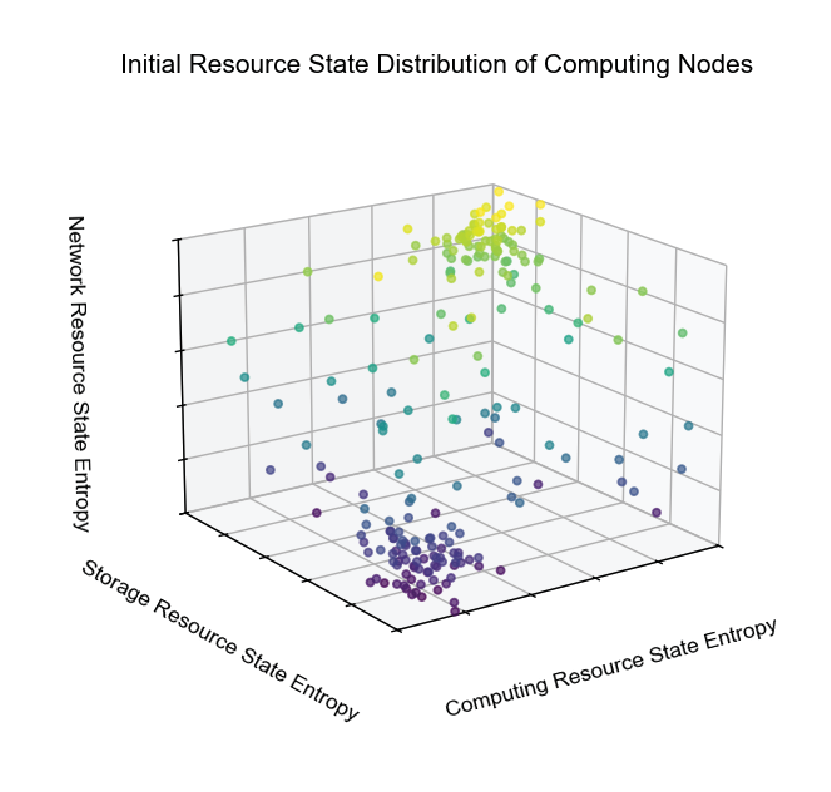
\includegraphics[width=0.85\columnwidth]{figures/figure2.eps}
	\caption{Initial resource state distribution of computing nodes.}
	\label{fig:initial_state}
\end{figure}

In the IoC, entropy-balanced matching aims to minimize the impact of task uncertainty and volatility on the state stability of the nodes represented by the resource matrix $\mathbf{R}$. In particular, variations in task arrival frequency and service time should have minimal effects on resource-state stability. Achieving this objective requires network-wide task--resource matching and scheduling.

When task $\mathbf{t}_i$ is well aligned with resource node $\mathbf{r}_j$ in the
resource space, the node remains relatively stable, resulting in low
single-node entropy and a globally balanced state. Conversely, a
substantial mismatch increases node-state fluctuations, leading to
high local entropy and global imbalance.

To achieve entropy balance, the scheduling strategy is implemented in
two steps.

First, the scheduler maintains the stability of individual node entropy among the nodes represented by the resource matrix $\mathbf{R}$. It calculates the expected squared distance between task $\mathbf{t}_i(c_i,l_i,s_i)$ and each candidate node $\mathbf{r}_j(c_j,l_j,s_j)$, and selects the node $\mathbf{r}_{\min}$ with the minimum expected squared distance for task matching and scheduling. This selection minimizes the state fluctuation caused by task allocation.
\begin{equation}
	\begin{aligned}
		\mathbf{r}_{\min}
		&= \operatorname*{arg\,min}_{\mathbf{r}_j:\,1\le j\le N}
		D(\mathbf{t}_i,\mathbf{r}_j) \\
		&= \operatorname*{arg\,min}_{\mathbf{r}_j:\,1\le j\le N}
		\mathrm{E}\!\left[
		\left\|\mathbf{t}_i-\mathbf{r}_j\right\|_2^2
		\right].
	\end{aligned}
	\label{eq:min_variance_matching}
\end{equation}

Second, to promote overall entropy balance across the nodes represented by the resource matrix $\mathbf{R}$, if $W$ nodes have expected squared task--resource distances close to the minimum within a predefined interval, they form the candidate set $\mathcal{C}_i$. The node with the minimum squared deviation between its comprehensive resource-state entropy and the balanced entropy is prioritized for selection. If the balanced entropy is set to 0.469, the selection rule is expressed as follows:
\begin{equation}
	\begin{aligned}
		\mathbf{r}_*
		&= \operatorname*{arg\,min}_{\mathbf{r}_j\in\mathcal{C}_i}
		D\!\left(H(\mathbf{r}_j),0.469\right) \\
		&= \operatorname*{arg\,min}_{\mathbf{r}_j\in\mathcal{C}_i}
		\left(H(\mathbf{r}_j)-0.469\right)^2.
	\end{aligned}
	\label{eq:entropy_balance_selection}
\end{equation}

If the selected node $\mathbf{r}_*$ belongs to service provider A, the task is scheduled across regions within A's resource pool. If the node belongs to another computing service provider B, interconnection between the resources of A and B is established, and the task is assigned to B through cross-regional or cross-entity scheduling.

If the task state deviates substantially from the available resource states, or if the candidate nodes' comprehensive entropy deviates substantially from the balanced entropy, new computing nodes may be planned to satisfy its requirements.

Figure~\ref{fig:matching_result} shows the resource-state distribution
after applying the proposed matching and scheduling mechanism to the
initial state in Figure~\ref{fig:initial_state}. The three marker types
represent training, inference, and rendering tasks, each forming a
concentrated region in the three-dimensional resource-state space.

Based on the entropy distributions in
Tables~\ref{tab:computing-resource-entropy},
\ref{tab:network-resource-entropy}, and
\ref{tab:storage-resource-entropy}, the system matches resources to
task-specific requirements. Nodes assigned to the same task type
occupy nearby positions in the entropy space, maintaining both
individual-node stability and network-wide entropy balance.
\begin{figure}[!t]
	\centering
	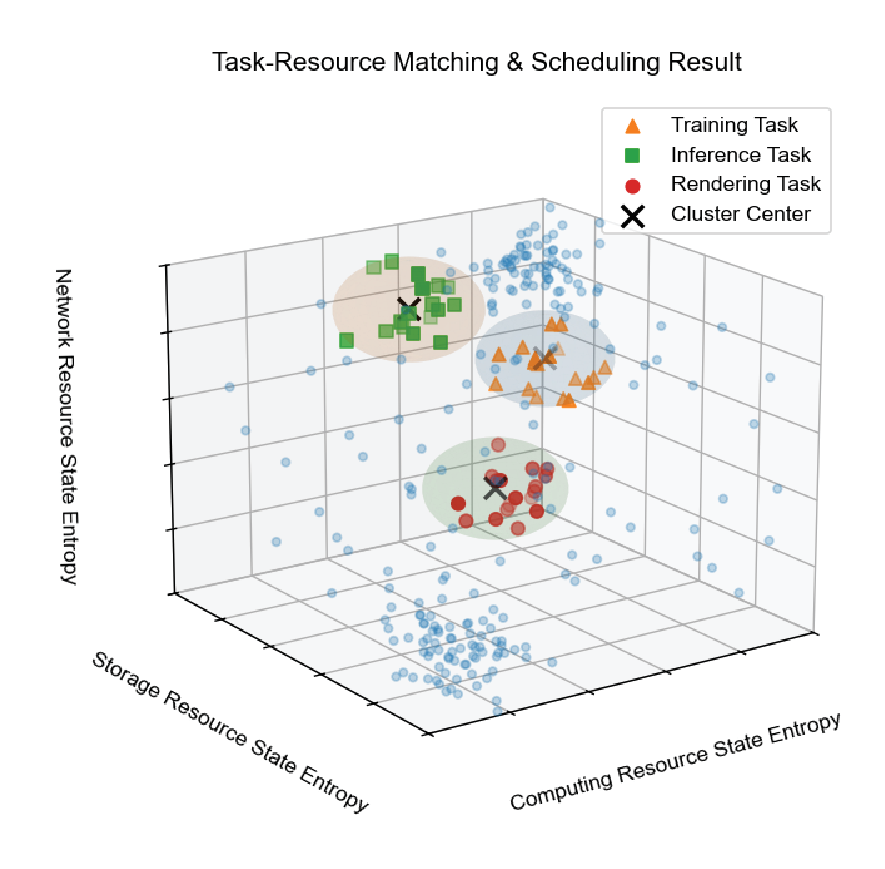
\includegraphics[width=0.80\columnwidth]{figures/figure3.eps}
	\caption{Resource distribution after task matching and scheduling.}
	\label{fig:matching_result}
\end{figure}

\subsection{Network Capacity Model}
\label{s3-6}

Resource matching in the IoC requires joint consideration of computing-resource availability and inter-node network performance. Scheduling solely according to computing load may overlook the effects of network bandwidth utilization and network latency on data synchronization. To address this limitation, this paper proposes a network capacity model that combines effective remote bandwidth with the entropy balance mechanism. The model quantifies the service capability of long-distance network links and supports task allocation in heterogeneous and dynamic environments.

The effective remote bandwidth is expressed as follows:
\begin{equation}
	\begin{aligned}
		C_{net}
		&= \text{Effective Remote Bandwidth} \\
		&= \frac{D}
		{T_{\text{remote}}-N_{\text{LD}}\cdot RTT}
		\times{\eta},
	\end{aligned}
	\label{eq:effective_remote_bandwidth}
\end{equation}
where
\begin{itemize}[nosep]
	\item $C_{net}$ denotes the network capacity model;
	
	\item $D$ denotes the volume of data to be transmitted;
	
	\item $T_{\text{remote}}$ denotes the observed end-to-end time required to complete the data transmission;
	
	\item $N_{\text{LD}}$ denotes the number of long-distance communications;
	
	\item $RTT$ denotes the round-trip time of the link;
	
	\item $\eta$ ($0<\eta\leqslant1$) denotes the bandwidth utilization factor.
\end{itemize}

Network capacity represents the effective data rate after fixed network latency is excluded. It captures the combined effects of physical bandwidth, protocol efficiency, link reliability, and concurrent-task interference, thereby dynamically reflecting the actual service capability of RDMA dedicated lines in multi-tenant and multi-task environments.

The utilization factor $\eta$ is not constant and varies with protocol overhead, congestion control, packet loss, and dynamic interference from coexisting traffic. In particular, even when RDMA dedicated lines are used and the physical links are dedicated to high-performance computing traffic, multiple parallel jobs may still share the underlying bandwidth. This sharing causes bandwidth convergence and intra-channel interference among concurrent jobs, which can be analogized to noise in network. Although such interference does not compromise data integrity, it can substantially reduce the effective throughput of the target flow. Consequently, the actual single-flow bandwidth may remain below the physical upper limit and vary with the system load. Therefore, $\eta$ should be monitored in real time to reflect changes in the operating conditions of RDMA dedicated lines.

During task matching, the scheduler uses historical or real-time measurements of $C_{net}$ to determine whether the network links between candidate nodes satisfy the data synchronization requirements of a task. For gradient-synchronization-intensive distributed training, the scheduler avoids node pairs whose $C_{net}$ is below the required threshold. Such paths are excluded even when computing resources are available, preventing network from becoming a performance bottleneck. The model supports resource matching in large-scale, cross-domain, and high-concurrency computing scenarios.

\section{Architecture of the IoC}
\label{s4}

\subsection{System Architecture}
\label{s4-1}

In the traditional Internet architecture, the bearer network and service network are loosely coupled, as shown in Figure~\ref{fig:Comparison of the System Architecture}. The bearer network is responsible for packet forwarding and transmission, without separating the control plane from the transport plane, while the service network is deployed above it to support Over-The-Top (OTT) applications~\cite{25}. Because the bearer network cannot perceive upper-layer application states, it cannot effectively coordinate computing resources with network conditions. This limitation becomes increasingly evident in scenarios such as AI training and inference, which require close coordination between computing and network resources.

\begin{figure}[!htbp]
	\centering
	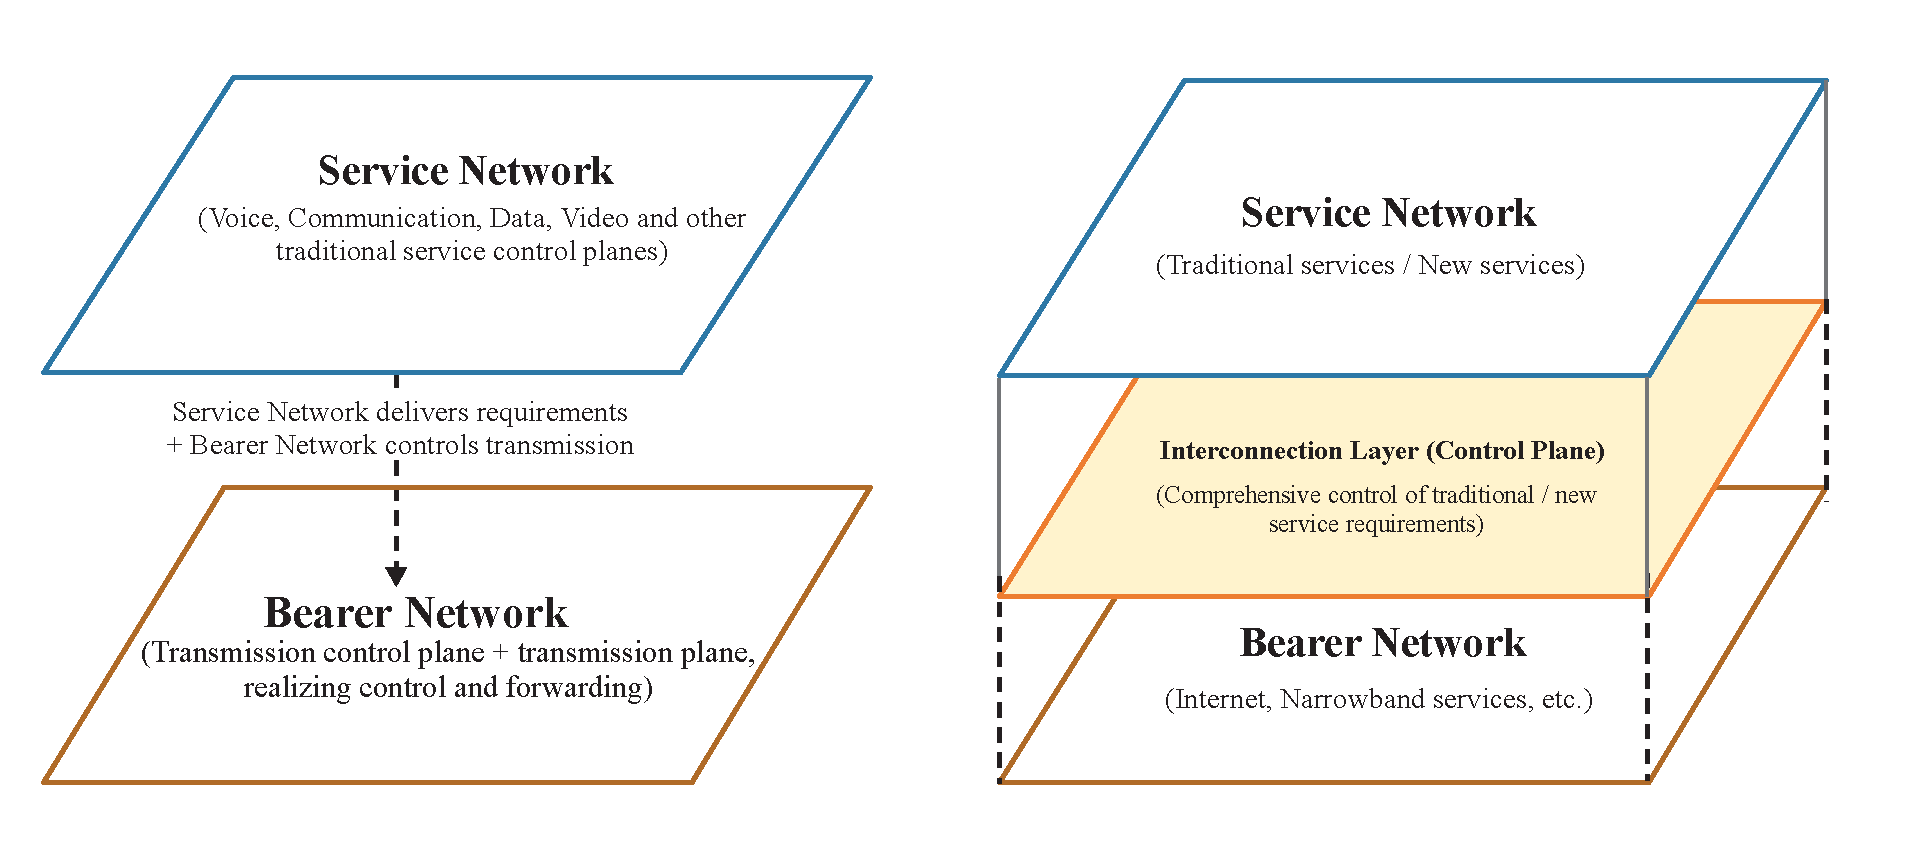
\includegraphics[width=0.90\columnwidth]{figures/figure4.eps}
	\caption{Comparison between the IoC and traditional Internet architectures.}
	\label{fig:Comparison of the System Architecture}
\end{figure}

Building on the previously proposed IoC architecture, this paper adopts a three-tier system comprising the Compute and Network Infrastructure Layer, Interconnection Resource Layer, and Application Service Layer. The architecture integrates computing services with the bearer network, as shown in Figure~\ref{fig:three-tier-architecture}. Its key enhancement is the Interconnection Resource Layer, which separates the control plane from the bearer network and integrates network control with computing-service control. This layer enables unified abstraction and perception of computing and network resources, together with network-wide task--resource matching and scheduling.

\subsubsection{Networking Architecture}
\label{s4-1-1}

As shown in Figure~\ref{fig:three-tier-architecture}, the networking architecture comprises the Compute and Network Infrastructure Layer, Interconnection Resource Layer, and Application Service Layer. This layered design organizes system functions according to service requirements and improves architectural adaptability.

\begin{figure}[!htbp]
	\centering
	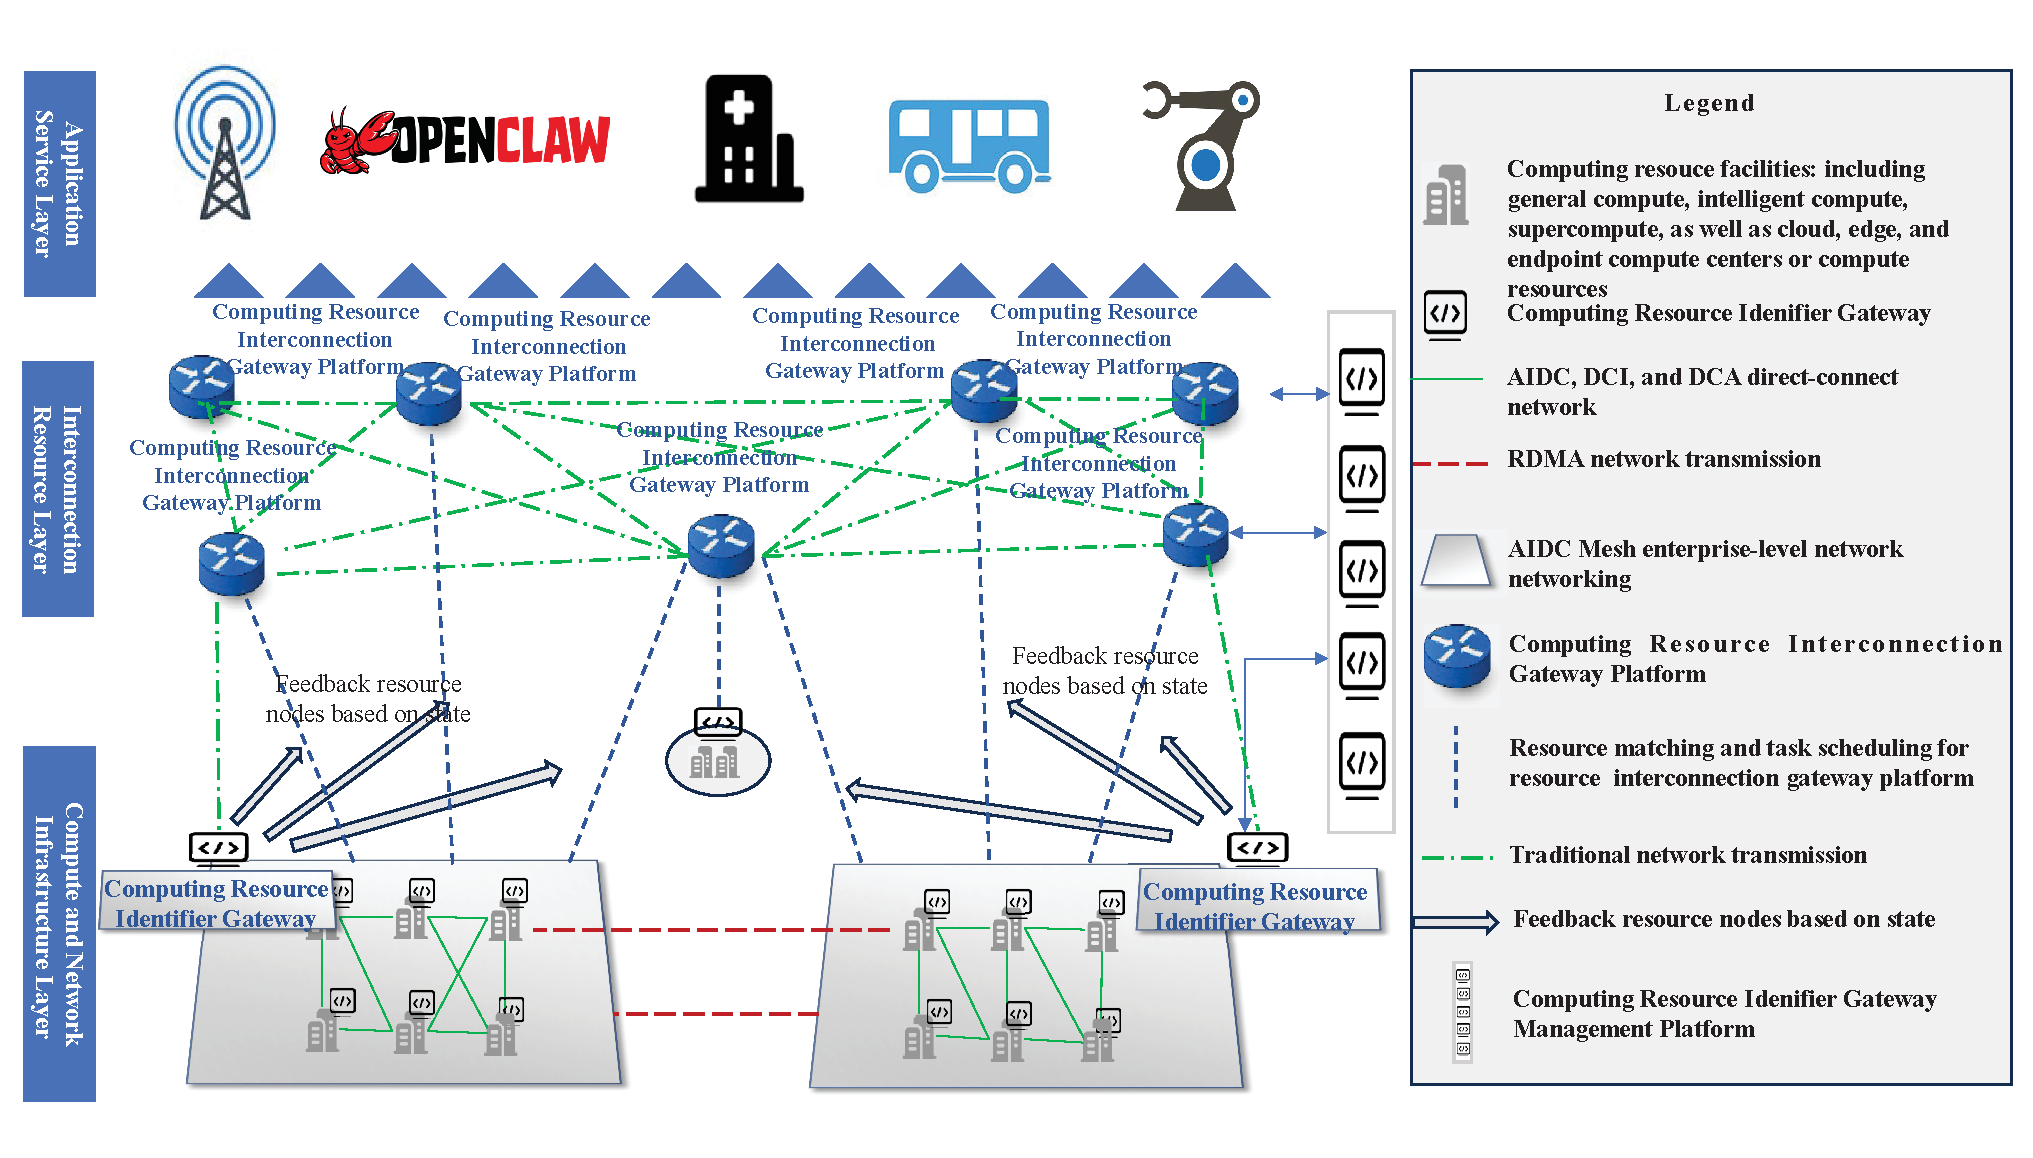
\includegraphics[width=0.90\columnwidth]{figures/figure5.eps}
	\caption{Three-tier architecture of the IoC.}
	\label{fig:three-tier-architecture}
\end{figure}

\subsubsection{Protocol Architecture}
\label{s4-1-2}

The IoC protocol architecture builds on the five-layer Internet model to maintain compatibility with the existing Internet architecture. At the transport layer, it enhances high-performance transmission through technologies such as RDMA. At the application layer, it extends computing-task data protocols and CRIDs to support task identification and resource-aware transmission over RDMA, as shown in Figure~\ref{fig: Protocol Architecture of the IoC}.

\begin{figure}[!htbp]
	\centering
	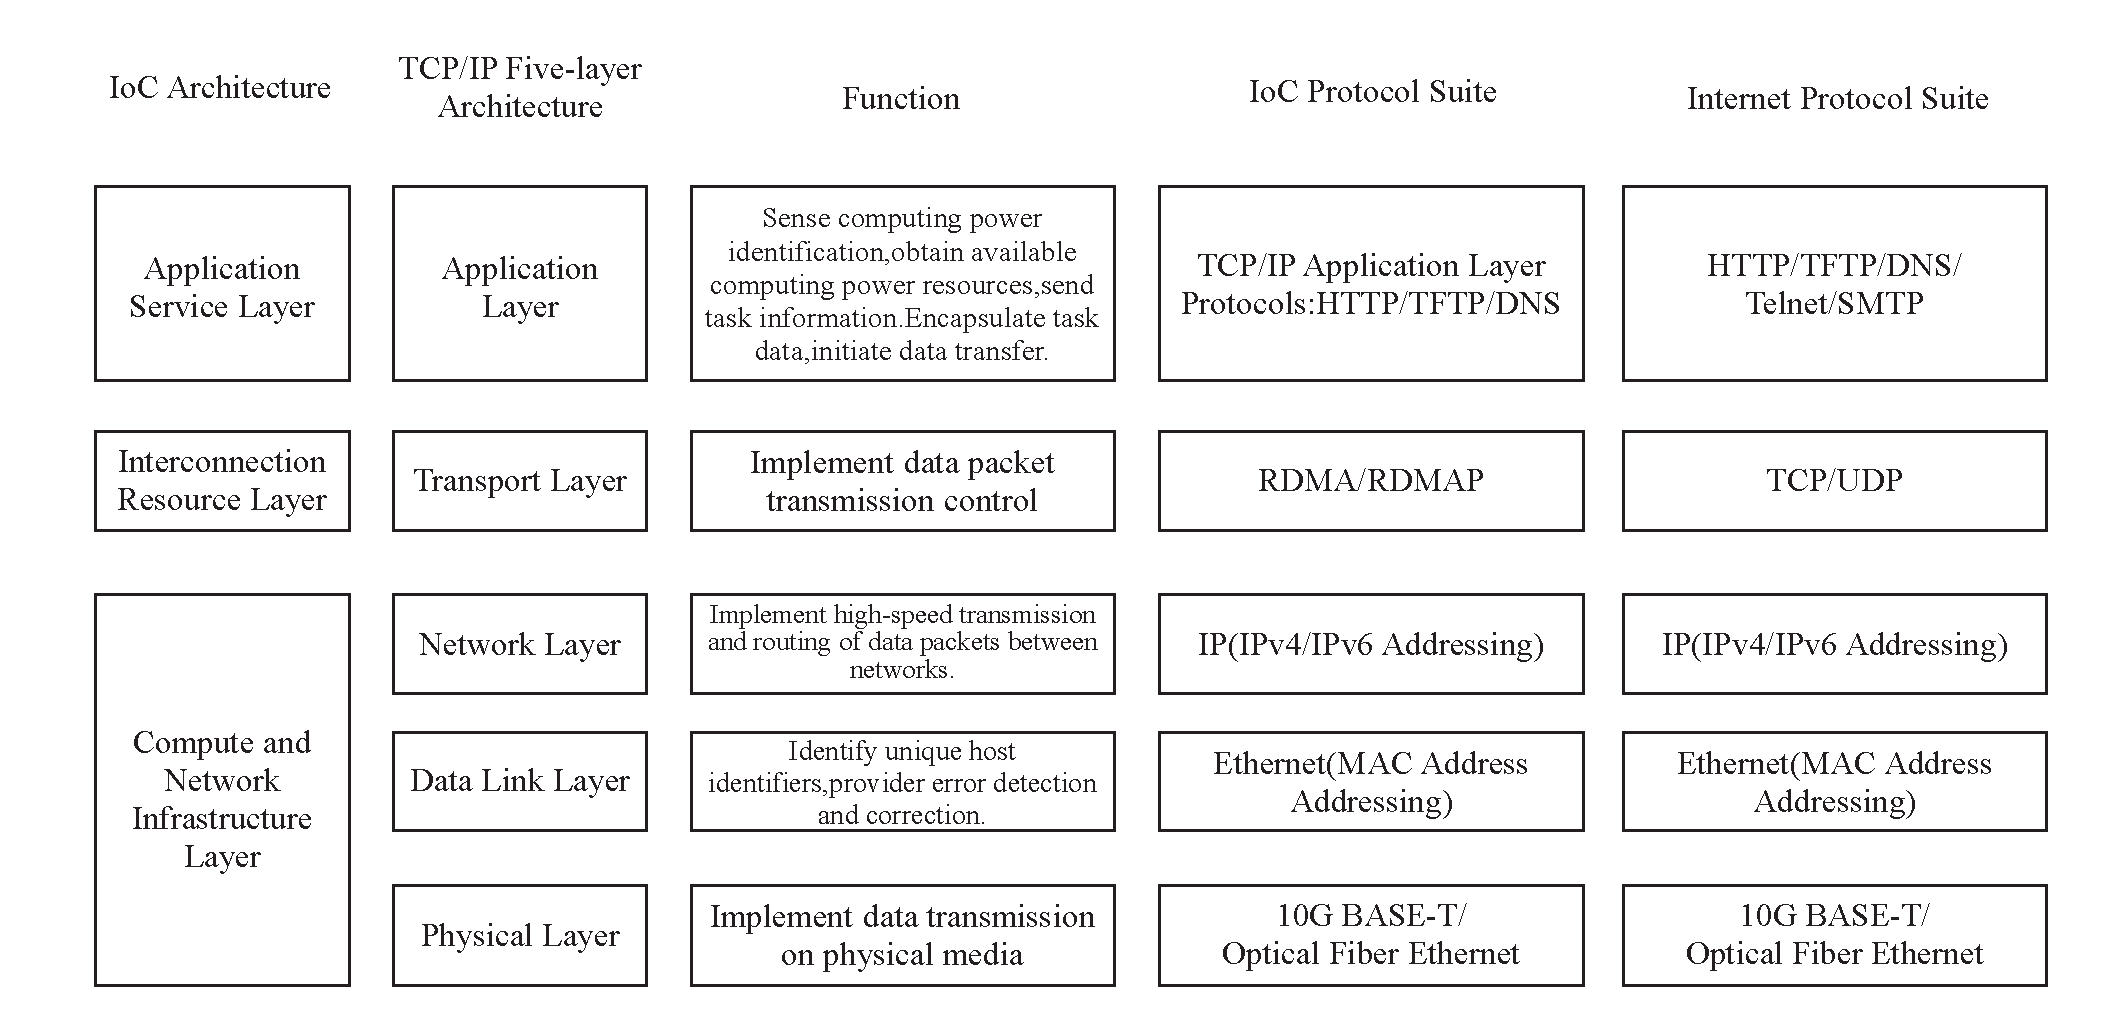
\includegraphics[width=1.00\columnwidth]{figures/figure6.eps}
	\caption{Protocol architecture of the IoC.}
	\label{fig: Protocol Architecture of the IoC}
\end{figure}

\subsection{Compute and Network Infrastructure Layer}
\label{s4-2}

\subsubsection{Optical Bearer Network}
\label{s4-2-1}

The Compute and Network Infrastructure Layer provides the physical resources required for computation and data transmission. Computing infrastructure includes general-purpose, intelligent, and supercomputing resources distributed across data centers, cloud platforms, and edge environments. Transmission infrastructure interconnects these resources through enterprise-level data-center connections~\cite{26}, mesh networks~\cite{27}, and the traditional Internet. Optical bearer networks provide the high-capacity transmission foundation for these interconnection modes.

\subsubsection{Compute Cloud Private Network}
\label{s4-2-2}

The Compute Cloud Private Network provides high-bandwidth, low-latency, and highly reliable interconnection among computing resources. It is typically constructed using Optical Transport Network/Wavelength Division Multiplexing (OTN/WDM), core routing and switching, and Data Center Interconnection (DCI). These technologies connect geographically distributed data centers, computing clusters, and edge nodes, supporting cross-domain resource sharing and elastic scheduling. Technologies such as SRv6, IPv6+, and network slicing further improve resource-orchestration precision and service determinism while enabling integration with cloud-network platforms and edge-computing systems. Together, these capabilities support integrated computing-resource scheduling and the development of a sustainable computing and network ecosystem.

\subsection{Interconnection Resource Layer}
\label{s4-3}

The Interconnection Resource Layer enables unified orchestration and scheduling of computing, storage, and network resources. It consists of three main components: the CRID Gateway, the RDMAP, and the entropy-balanced scheduling algorithm. By deploying CRID gateways, this layer enables network-wide resource-state perception. The resource state of node $i$ is represented as
\begin{equation}
	\label{eq:resource-status}
	\mathbf{r}_i = \mathbf{r}_i (c_i, l_i, s_i ),
\end{equation}
where $c_i$, $l_i$, and $s_i$ denote the computing, network, and storage states of the node, respectively.

Based on the perceived resource states, the Interconnection Resource
Layer provides interfaces for resource identification, resolution,
retrieval, query, and path-scheduling parameters, supporting the on-demand
use of heterogeneous resources by industries and enterprises. The
scheduling algorithm then matches computing tasks with appropriate
resources.

\subsubsection{The Overall Architecture of CRID}
\label{s4-3-1}

A unified identifier system for the IoC must extend beyond traditional static and flat addressing to represent the spatiotemporal attributes and dynamic states of computing resources. To this end, this paper proposes the CRID, which supports five-level positioning and addressing across enterprise, city, computing center, server, and chip, as shown in Figure~\ref{fig:crid-architecture}.

\begin{figure}[!ht]
	\centering
	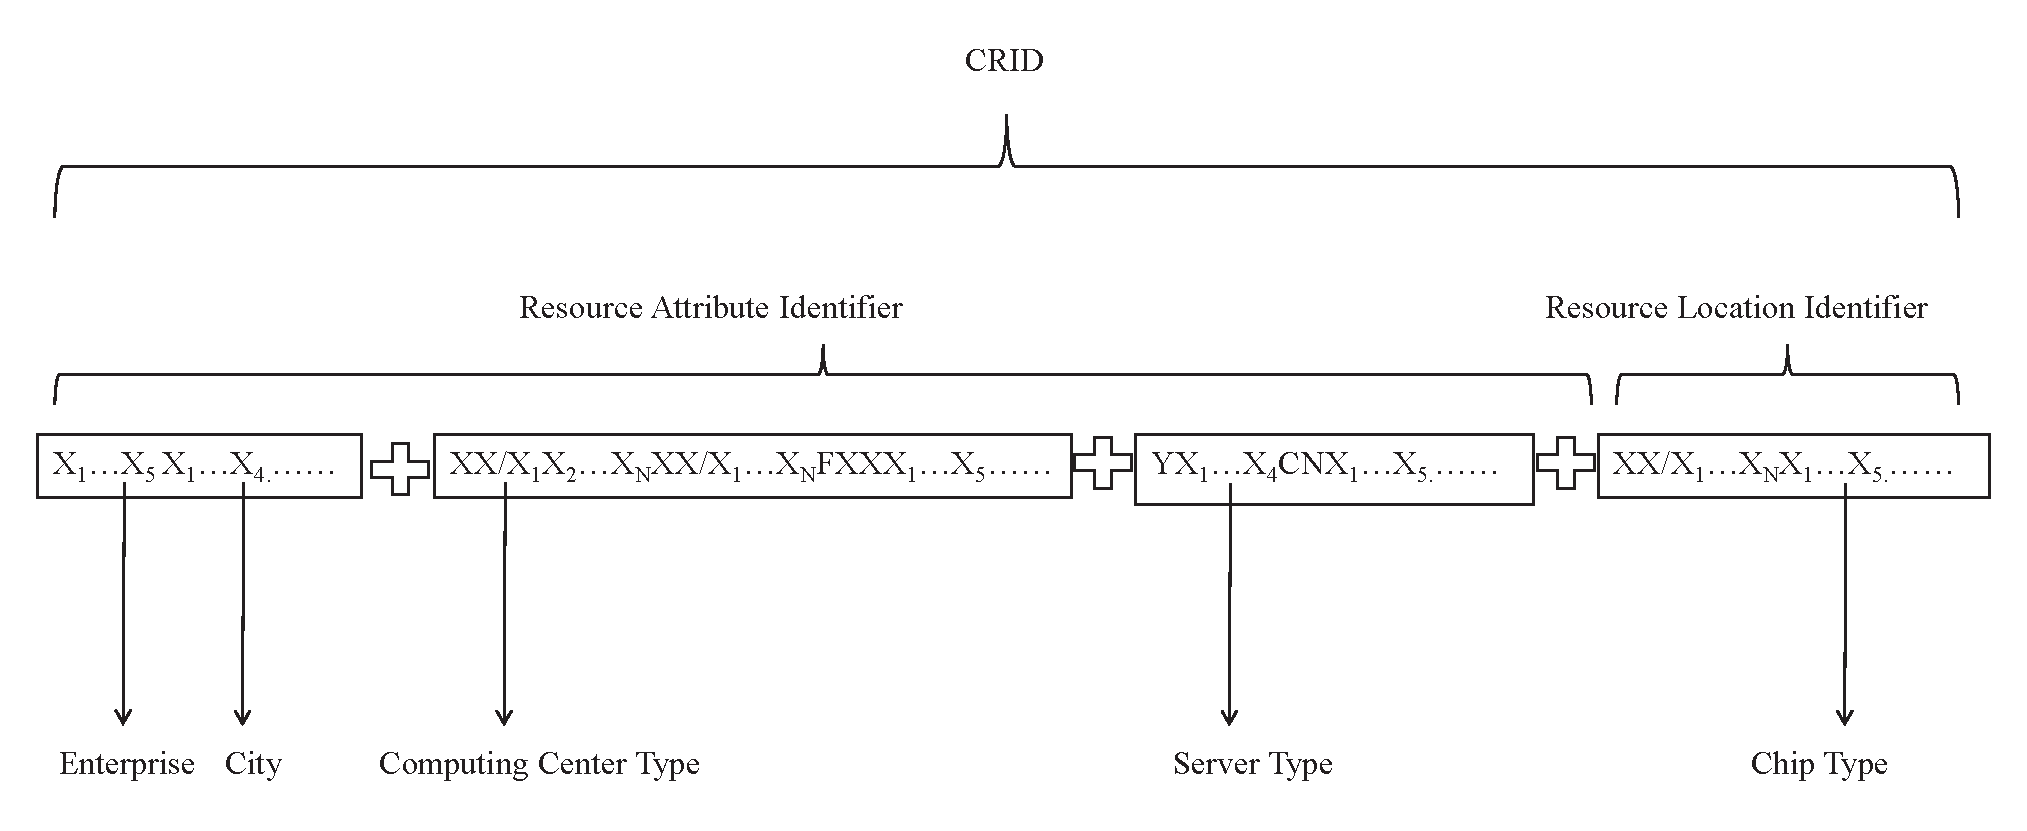
\includegraphics[width=0.90\columnwidth]{figures/figure7.eps}
	\caption{Overall architecture of the CRID.}
	\label{fig:crid-architecture}
\end{figure}

The CRID Gateway collects and calculates the computing utilization
$c_i$, storage utilization $s_i$, and inter-node network
utilization $l_i$ of each node, thereby forming the resource state
$\mathbf{r}_i(c_i,l_i,s_i)$. These measurements provide a dynamic data basis
for global resource scheduling, task optimization, and system
coordination.

The CRID adopts a two-segment prefix--suffix encoding structure to describe resource attributes, scale, specifications, and paths. Combined with hierarchical resolution and dynamic verification, it enables the precise positioning and trusted authentication of distributed heterogeneous computing resources. CRID assigns each computing resource a unique identifier and supports resource description, positioning, addressing, and utilization-state perception.

As the core component of the CRID system, the gateway collects,
verifies, resolves, and queries resource identifiers. It also
generates unique task identifiers to support intelligent
“task--resource” matching and entropy-balanced scheduling. At the
data-collection level, the gateway perceives and evaluates three
categories of node resources:

\begin{itemize}[nosep]
	\item Computing resources:
	The gateway collects the computing load, chip type (e.g., CPU, GPU,
	and TPU), chip model, chip count, core count, and memory capacity,
	providing the basis for calculating $c_i$;
	
	\item Storage resources:
	The gateway collects the storage architecture (e.g., distributed
	or centralized) and storage capacity, providing the basis for
	calculating $s_i$;
	
	\item Network resources:
	The gateway collects real-time information on network type,
	bandwidth capacity, and latency, and continuously monitors link
	stability and network efficiency, providing the basis for
	calculating $l_i$.
\end{itemize}

Based on the collected resource information, the gateway dynamically evaluates the computing, network, storage, and comprehensive state entropy of each node. The comprehensive state entropy is expressed as
\begin{equation}
	H(\mathbf{r}_i)=F\left(H(c_i),H(l_i),H(s_i)\right),
	\label{eq:comprehensive-entropy}
\end{equation}
where $F(\cdot)$ denotes the entropy fusion function for computing,
network, and storage resources.

The result with the minimum entropy fluctuation is fed back to the entropy calculation module when the next task arrives. Through this feedback reinforcement mechanism, both the accuracy and environmental adaptability of the entropy-balanced scheduling algorithm can be continuously improved.

\subsubsection{High-Performance Transmission Protocol}
\label{s4-3-2}

Traditional computing networks face decentralized resource scheduling, inefficient resource access, and limited traffic-control precision. To address these limitations, this paper proposes the RDMAP, a memory-access protocol framework extended from RDMA over Converged Ethernet v2 (RoCEv2). By deeply integrating CRIDs, RDMAP enables fine-grained perception and precise regulation of cross-domain traffic. It improves the computing efficiency ratio through coordinated resource scheduling and traffic management, promotes entropy balance within the network system, and enhances overall stability and resource utilization.

RoCEv2 provides high-performance, zero-copy data transmission.
Existing approaches extend the reserved bits of the Base Transport
Header (BTH) to carry additional path or scheduling information.
Conweave~\cite{32}, proposed by the National University of Singapore in 2023,
uses several BTH reserved bits as PathID/PathTag fields to identify
the uplink path assigned to each packet. This design enables explicit
and recoverable path selection, reducing receiver-side reordering
overhead and improving link utilization.

SeqBalance~\cite{33}, proposed by Huimin Luo et al. in 2024, uses the BTH
reserved bits to perform sequence- or tag-based traffic balancing and
support rapid forwarding decisions at network devices. It distributes
packets across multiple paths while preserving in-order semantics or
minimizing packet reordering.

Inter-node network in the IoC requires both efficient data
transmission and awareness of the remote computing state. RDMAP therefore extends the
protocol semantics of RoCEv2 while maintaining compatibility with its
basic transmission mechanism. This extension gives computing
resources global addressing and dynamic binding capabilities, allowing
existing RDMA devices to enable compute-aware transmission through
lightweight upgrades.

In terms of frame structure, RDMAP retains the basic RoCEv2 format and introduces lightweight extensions to the BTH reserved bits. One bit is used as the RDMAP flag, where 0 indicates a standard RoCEv2 frame and 1 indicates an RDMAP frame. A new RDMAP Header is inserted before the payload. The header contains a 1-byte start and end identifier and the CRID, embedding computing information into data packets to support long-distance computing--network collaboration, as shown in Figure~\ref{fig: RDMAP Frame Structure}.

\begin{figure}[!ht]
	\centering
	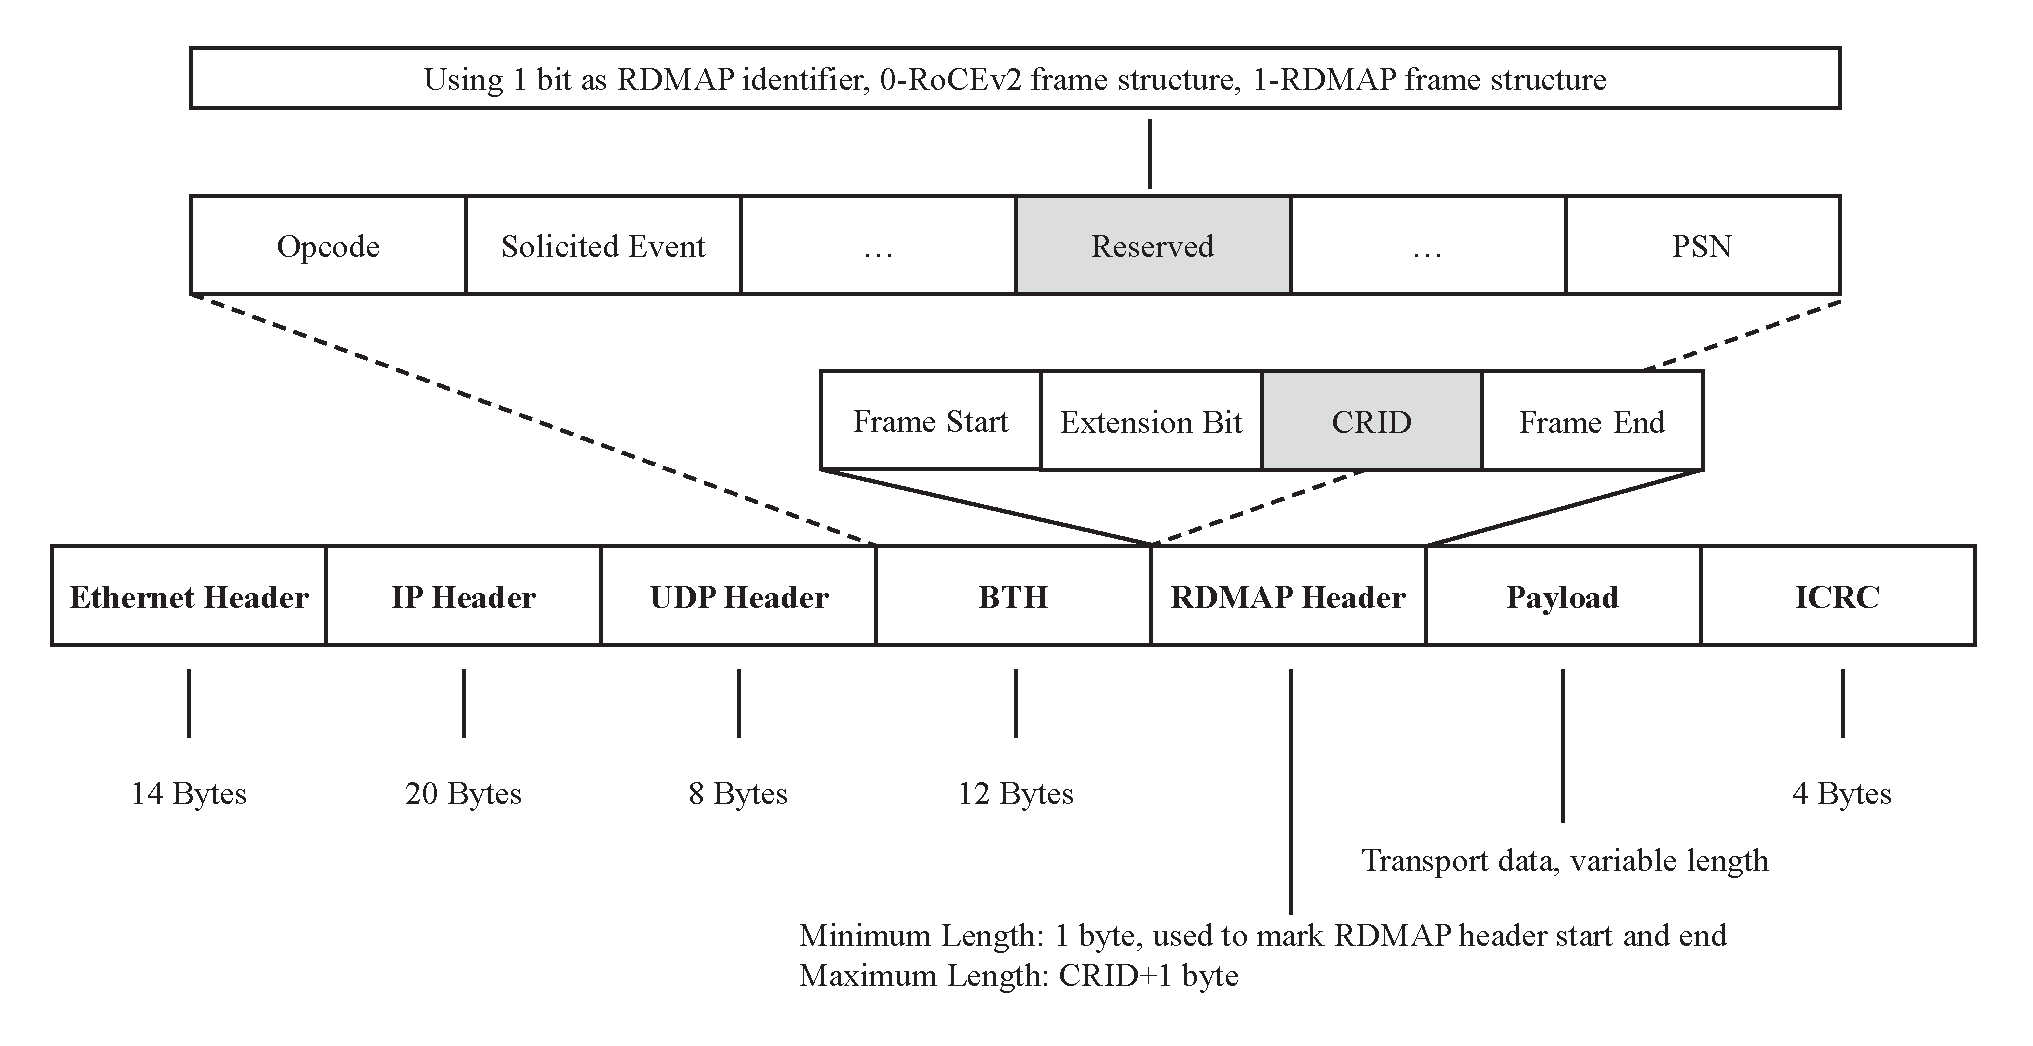
\includegraphics[width=1.00\columnwidth]{figures/figure9.eps}
	\caption{RDMAP frame structure.}
	\label{fig: RDMAP Frame Structure}
\end{figure}

\subsubsection{Scheduling Algorithm}
\label{s4-3-3}

The computing-resource scheduling algorithm matches different types
of computing tasks with optimal resources. It focuses on two
representative workloads: training and inference. Their distinct
computing characteristics and scheduling objectives require
differentiated strategies, providing the basis for subsequent
scheduling models and algorithms.

As artificial intelligence models continue to grow, the computing
requirements of training and inference tasks increase accordingly. A
single node or local data center may struggle to simultaneously
provide elastic resources, low-latency responses, and energy-efficient
operation.

Training tasks are compute-intensive and long-running, with strong
requirements for GPU performance and energy efficiency. Inappropriate
resource allocation may cause prolonged node overload and reduced
execution efficiency. Inference tasks are short-lived and highly
concurrent, requiring low latency and rapid, elastic resource
allocation.

Computing-resource scheduling is therefore a joint optimization
problem involving heterogeneous tasks~\cite{23} and distributed
computing, storage, and network resources~\cite{24}. Its objective is
to balance task latency, energy constraints, and resource
utilization~\cite{29}. Unlike traditional network routing, computing
scheduling emphasizes joint decision-making across multiple resource
dimensions and elastic resource orchestration.

The scheduling process consists of two steps.
\par
\Needspace{3\baselineskip}
\noindent 1) \textit{State Types and State Entropy Parameter Settings.}\par

The algorithm decomposes each task, analyzes the computing, network,
and storage requirements of its subtasks, and evaluates the states of
available computing nodes.

Based on the resource state entropy model, the algorithm considers
three scheduling factors: computing state $c$, network state
$l$, and storage state $s$. These factors represent the available
computing capability, inter-node network condition, and storage
capacity for caching or intermediate results, respectively.
\par
\Needspace{3\baselineskip}
\noindent 2) \textit{Weight Setting.}\par

Based on the global state entropy and entropy balance model, the comprehensive state entropy $H(\mathbf{r}_i)$ of resource node $\mathbf{r}_i$ is calculated according to Eq.~\eqref{eq:comprehensive_entropy}. The resource weights can be dynamically adjusted according to specific scenario requirements.

\section{Application Scenarios of the IoC}
\label{s5}

\subsection{LLM Training}
\label{s5-1}

\noindent In the IoC scenario, LLM training can utilize cross-domain heterogeneous resources to achieve efficient parallel computing. As shown in Figure~\ref{fig:model-training-process}, the cross-domain heterogeneous training architecture consists of three layers: the Application Service Layer, Interconnection Resource Layer, and Compute and Network Infrastructure Layer.

\begin{figure}[!ht]
	\centering
	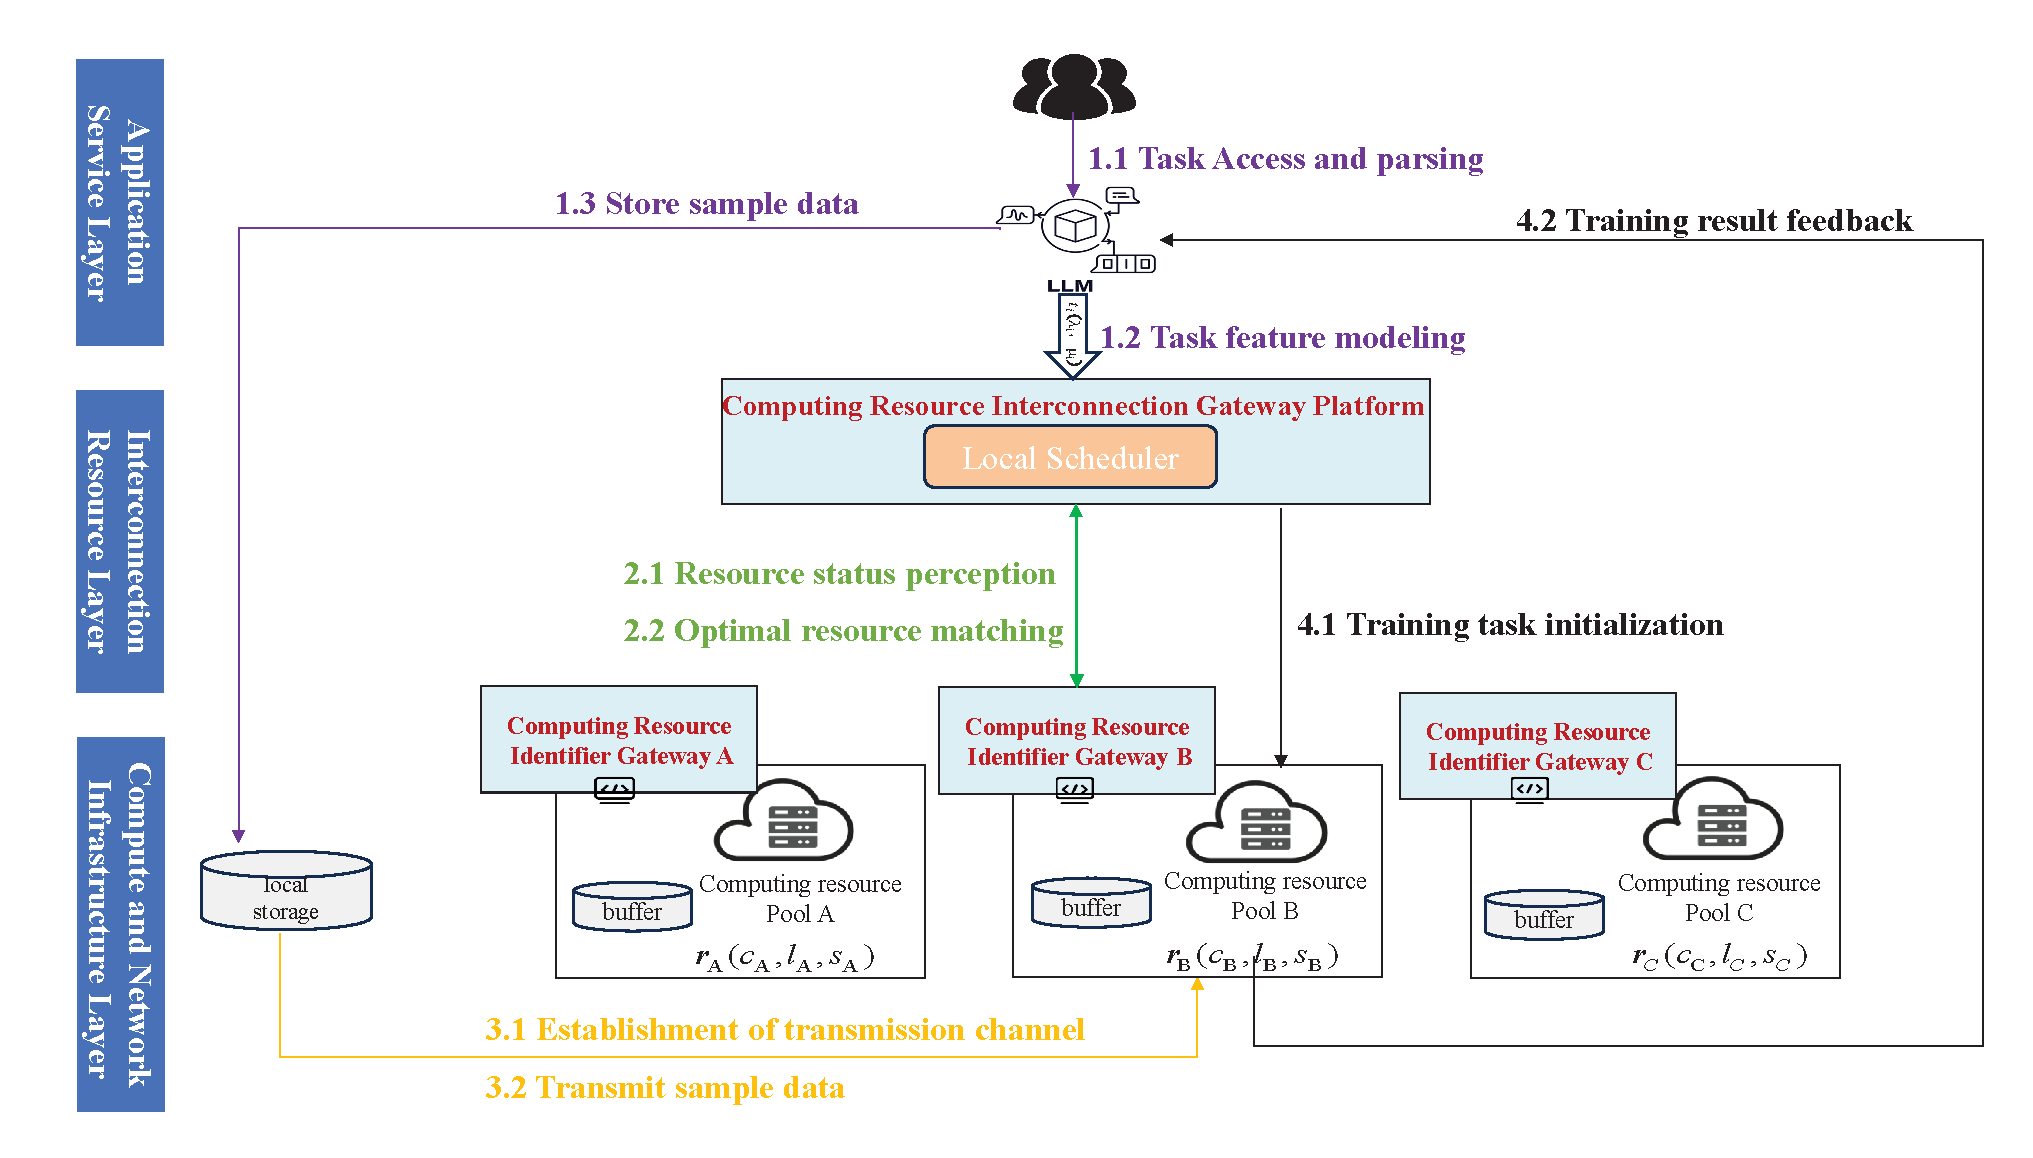
\includegraphics[width=0.90\columnwidth]{figures/figure10.eps}
	\caption{LLM training process in the IoC}
	\label{fig:model-training-process}
\end{figure}

\subsubsection{Training Architecture}
\label{s5-1-1}

First, the Application Service Layer describes training tasks, obtains the task parameters $\mathbf{t}_i(\lambda_i,\mu_i)$, and submits task requests to the Interconnection Resource Layer. The task description includes computing, storage, and network parameters.

\begin{itemize}[nosep]
	\item Computing parameters: Training sample size, model parameter size, number of training epochs, batch size, training/validation/testing ratios, and duration per training epoch, i.e., service time $\mu_i$.
	
	\item Storage parameters: Total cached sample data volume and incremental sample data volume per arrival.
	
	\item Network parameters: Incremental sample volume per arrival, i.e., the transmitted sample data volume, computing network capacity $C_{\text{net}}$, and arrival-time distribution $\lambda_i$.
\end{itemize}

Second, the Interconnection Resource Layer receives task requests, obtains the task parameters $\mathbf{t}_i(\lambda_i,\mu_i)$, uniformly encapsulates the tasks, and provides task-scheduling capabilities. By perceiving the underlying resource states $\mathbf{r}_i(c_i,l_i,s_i)$ through the CRID Gateway, this layer matches resource states with task requirements.

\begin{itemize}[nosep]
	\item CRID Gateway: Collects computing, storage, and network parameters and continuously monitors changes in the state $\mathbf{r}_i(c_i,l_i,s_i)$ of the selected resource nodes.
	
	\item RDMAP Transmission Control: After the CRID Gateway filters the computing nodes, RDMAP provides long-distance lossless transmission based on the RDMA protocol. It adjusts the transmission rate, congestion window, and traffic priority in real time according to the network capacity model and network resource state entropy, thereby ensuring data synchronization during LLM training.
	
	\item Scheduling Algorithm: Matches the task parameters $\mathbf{t}_i(\lambda_i,\mu_i)$ with the node state $\mathbf{r}_i(c_i,l_i,s_i)$ and accurately assigns training tasks to optimal computing nodes. It dynamically adjusts resource allocation according to real-time node states $\mathbf{r}_i(c_i,l_i,s_i)$, thereby maintaining balanced resource utilization during training.
\end{itemize}

Third, the Computing and Network Infrastructure Layer provides the physical infrastructure for task execution and data transmission. It provides the computing, storage, and network capabilities $\mathbf{r}_i(c_i,l_i,s_i)$ of interconnected heterogeneous resource nodes and synchronizes their capabilities and states with the Interconnection Resource Layer in real time.

\begin{itemize}[nosep]
	\item Computing Resources: The core computing resources for distributed LLM training consist of heterogeneous intelligent computing nodes optimized for AI training scenarios.
	
	\item Storage Resources: Local node storage and remote resource-pool storage provide sample data and model parameters for LLM training.
	
	\item Network Resources: RDMA-based channels provide high-speed, lossless remote data transmission for training tasks.
\end{itemize}

\subsubsection{Training Process}
\label{s5-1-2}

The LLM training process in the IoC scenario consists of four core stages: training task identification, task--compute matching, training data transmission flow, and training task execution. The workflow of each stage is described below.

\par
\Needspace{3\baselineskip}
\noindent\textit{Training Task Identification.}\par

\begin{enumerate}[nosep,label=\arabic*)]
	\item Task Access and Parsing: The Application Service Layer receives user-initiated LLM training tasks, parses core parameters including training sample size, model parameter size, training epochs, and batch size, and extracts the corresponding computing, storage, and network requirements.
	
	\item Task Feature Modeling: Based on the parsed task parameters, the Application Service Layer performs statistical modeling of the training tasks and generates the task features $\mathbf{t}_i(\lambda_i,\mu_i)$. The task requests and feature vectors are then sent to the Gateway Platform of the Interconnection Resource Layer.
	
	\item Sample Data Storage: The Application Service Layer stores the training sample data in the local storage resource pool, completing data preparation before training execution.
\end{enumerate}

\par
\Needspace{3\baselineskip}
\noindent\textit{Task--Compute Matching.}\par

\begin{enumerate}[nosep,label=\arabic*)]
	\item Resource State Perception: the CRID Gateway of the Interconnection Resource Layer collects the real-time computing, storage, and network states of the three types of resource nodes (A, B, and C) in the Computing and Network Infrastructure Layer and synchronizes the state information with the Gateway Platform.
	
	\item Optimal Resource Matching: According to the task requirements and underlying resource states, the Gateway Platform applies the entropy-balanced scheduling algorithm to select the optimal node, such as Node C, from Nodes A, B, and C.
\end{enumerate}

\par
\Needspace{3\baselineskip}
\noindent\textit{Training Data Transmission Flow.}\par

\begin{enumerate}[nosep,label=\arabic*)]
	\item Transmission Channel Establishment: The Gateway Platform issues training-execution instructions to the selected target computing node and completes the standardized encapsulation and distribution of the training task. Meanwhile, the Interconnection Resource Layer establishes an end-to-end high-speed, lossless data-transmission channel between the local storage resource pool and the target computing node using the RDMAP protocol.
	
	\item Sample Data Transmission: The local storage resource pool transmits the pre-trained model weight files and training sample data to the target computing node, completing data-resource preparation before training execution.
\end{enumerate}

\par
\Needspace{3\baselineskip}
\noindent\textit{Training Task Execution.}\par

\begin{enumerate}[nosep,label=\arabic*)]
	\item Training Task Startup: After receiving the training instructions, the target computing node initializes the training environment, prefetches and loads training-sample batches through the RDMAP high-speed channel, and starts the training task.
	
	\item Training Result Return: Upon completing model training, the selected resource node transmits the final trained model parameters and results back to the Application Service Layer through the network.
\end{enumerate}


\subsection{LLM Inference}
\label{s5-2}

\subsubsection{Inference Architecture}
\label{s5-2-1}

\noindent In the IoC scenario, the demand for concurrent LLM inference has increased significantly. Multiple inference tasks can be processed by offloading them across heterogeneous resources in different domains, as shown in Figure~\ref{fig:model-inference-process}.

\begin{figure}[!ht]
	\centering
	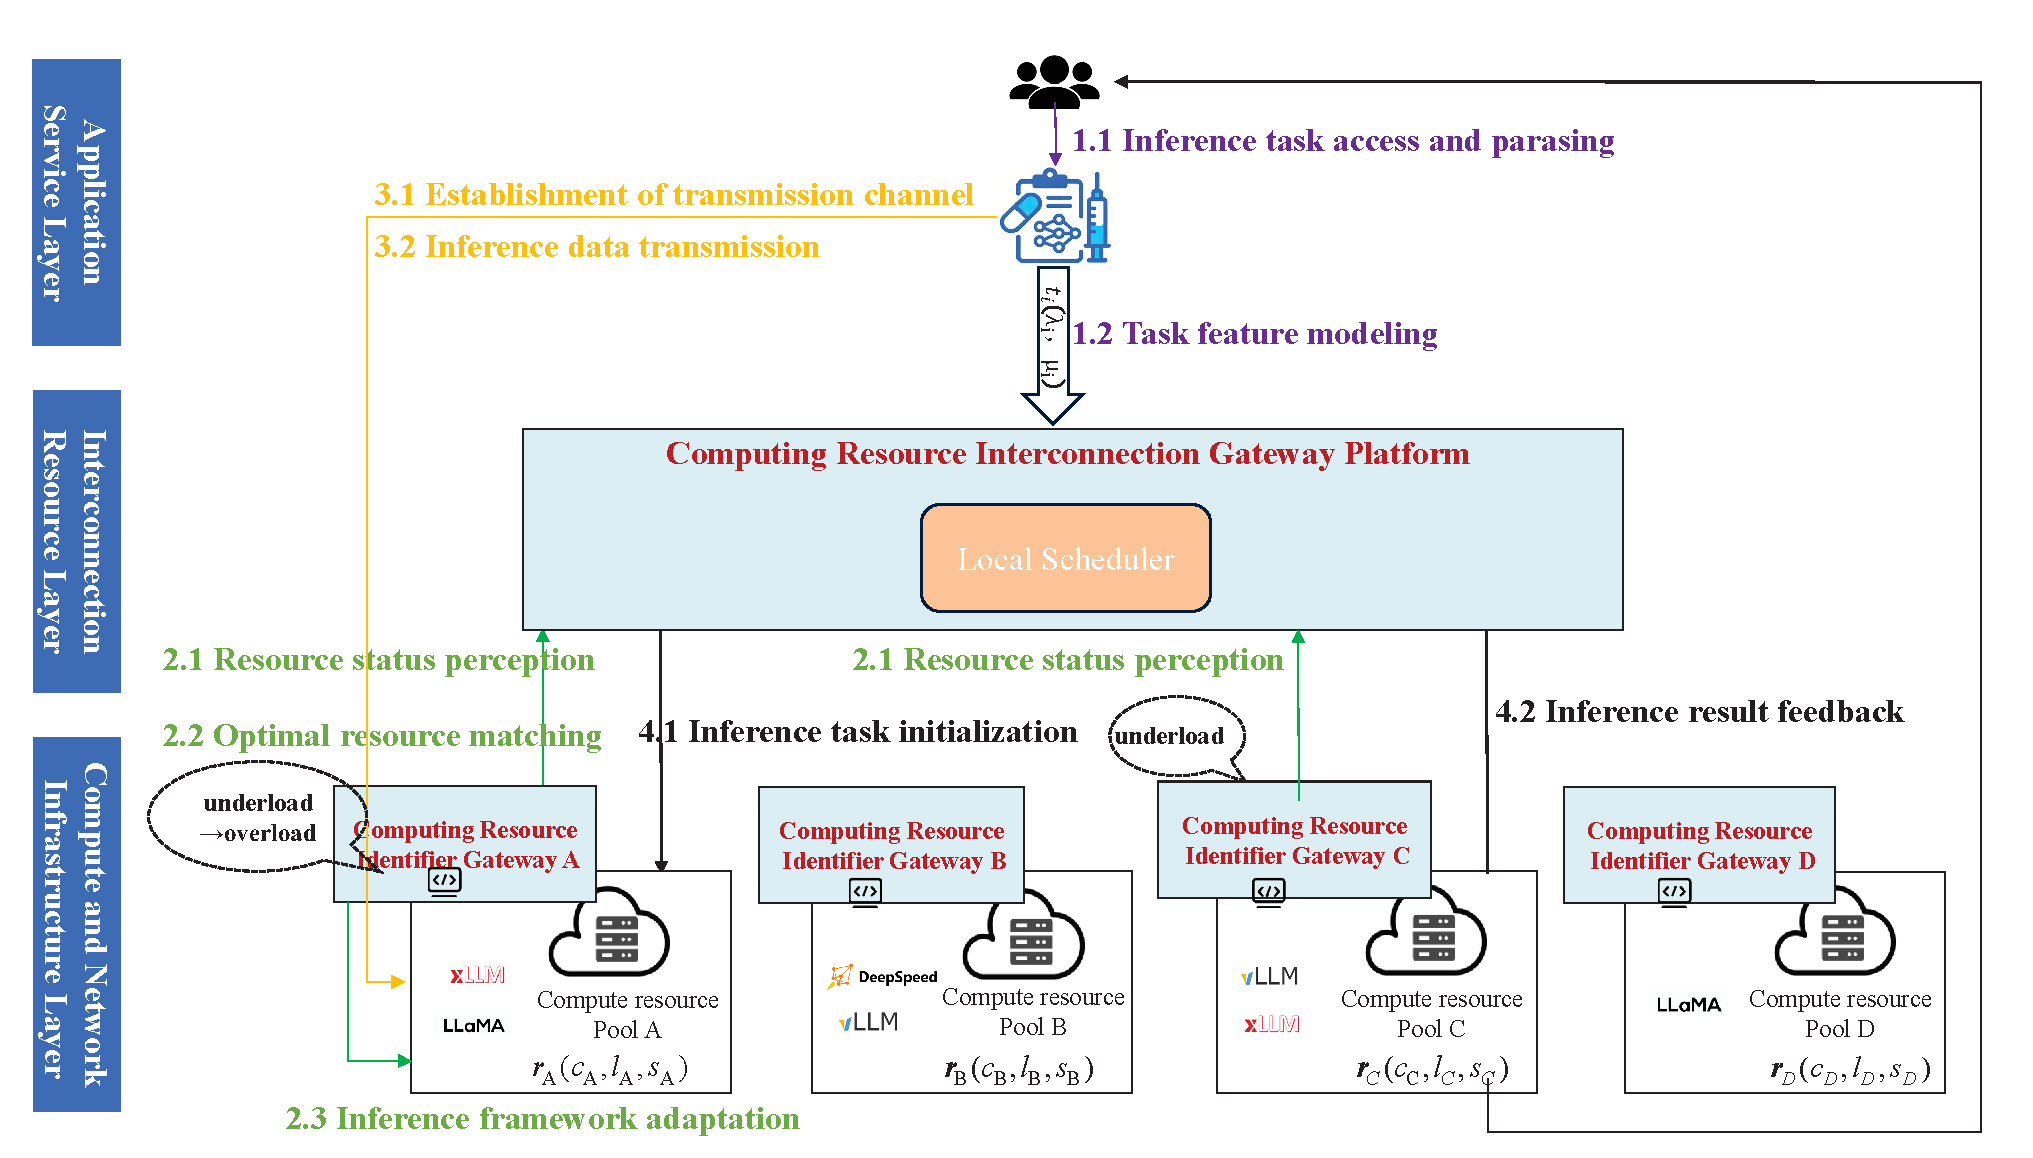
\includegraphics[width=0.90\columnwidth]{figures/figure11.eps}
	\caption{LLM inference process in the IoC}
	\label{fig:model-inference-process}
\end{figure}

First, the Application Service Layer serves inference scenarios such as intelligent question answering and multimodal generation. It parses and describes inference tasks, obtains the task parameters $\mathbf{t}_i(\lambda_i,\mu_i)$, and sends the resulting inference requests to the Interconnection Resource Layer.

\begin{itemize}[nosep]
	\item Computing parameters: Input prompt length, expected generated-content length, and model parameter scale.
	
	\item Storage parameters: Required model-parameter cache volume, selected-model weight size, and KV cache occupancy.
	
	\item Network parameters: Arrival-time distribution $\lambda_i$, transmitted data volume per request, and network bandwidth and latency requirements.
\end{itemize}

Second, the Interconnection Resource Layer uses the CRID Gateway to perceive the underlying resource states $\mathbf{r}_i(c_i,l_i,s_i)$. Based on these states and the inference task $\mathbf{t}_i(\lambda_i,\mu_i)$, model type, and underlying chip model, the layer selects resource nodes with optimal resource utilization and matches the optimal inference acceleration framework. The inference tasks are then distributed to the matched resource nodes to maintain balanced resource states and improve inference efficiency.

\begin{itemize}[nosep]
	\item CRID Gateway: Collects and updates the computing, storage, and network parameters of each node in real time, thereby continuously perceiving its resource state $\mathbf{r}_i(c_i,l_i,s_i)$.
	
	\item Scheduling Algorithm: Evaluates candidate resource states according to the latency and concurrency requirements of inference tasks and the task parameters $\mathbf{t}_i(\lambda_i,\mu_i)$, and continuously selects the optimal resource nodes for different inference tasks.
\end{itemize}

Third, the Computing and Network Infrastructure Layer provides computing resources, models, and inference acceleration frameworks across interconnected heterogeneous resource pools. The CRID Gateways deployed in these resource pools monitor their computing, storage, and network states $\mathbf{r}_i(c_i,l_i,s_i)$ in real time and synchronize the results with the Interconnection Resource Layer through interfaces. Based on the task--model matching results, the layer activates the deployed inference acceleration frameworks on the selected resource nodes to provide optimal inference acceleration.

\begin{itemize}[nosep]
	\item Computing Resources: Comprise heterogeneous intelligent computing nodes deeply optimized for AI scenarios and serve as the core computing carriers for distributed LLM inference.
	
	\item Inference Acceleration Frameworks: Multiple mainstream inference acceleration frameworks are pre-deployed to support different chip architectures and model types.
	
	\item Storage Resources: Distributed storage resource pools provide high-speed caching and storage for inference model parameters, hot request samples, and temporary inference results.
	
	\item Network Resources: Provide low-jitter and highly reliable transmission for cross-node inference task distribution, model weight synchronization, and inference result return.
\end{itemize}

\subsubsection{Inference Process}
\label{s5-2-2}

The LLM inference process in the IoC consists of four core stages: inference task identification, task-compute matching, inference data transmission flow, and inference task execution.

\par
\Needspace{3\baselineskip}
\noindent\textit{Inference Task Identification.}\par

\begin{enumerate}[nosep,label=\arabic*)]
	\item Inference Task Access and Parsing: The Application Service Layer receives inference requests and parses their core parameters.
	
	\item Task Feature Modeling: Based on task parameters such as the task arrival characteristic $\lambda_i$ and service time characteristic $\mu_i$, the Application Service Layer models each task to generate the task feature $\mathbf{t}_i(\lambda_i,\mu_i)$ and sends the generated feature to the Gateway Platform of the Interconnection Resource Layer.
\end{enumerate}

\par
\Needspace{3\baselineskip}
\noindent\textit{Task-Compute Matching.}\par

\begin{enumerate}[nosep,label=\arabic*)]
	\item Resource State Perception: Through the CRID Gateway deployed on each node, the Interconnection Resource Layer monitors the computing, network, and storage resource states and the deployed inference acceleration frameworks of all candidate resource nodes in the Compute and Network Infrastructure Layer in real time. Core parameters, including real-time node load, available computing capability, and link bandwidth, are collected and synchronized with the Gateway Platform.
	
	\item Optimal Resource Matching: The Gateway Platform runs the entropy-balanced scheduling algorithm and jointly considers task requirements and node resource states. It selects the optimal inference node from the cross-domain candidate resource pools according to resource-state stability and task--resource compatibility, and then issues the inference execution instructions.
	
	\item Inference Framework Adaptation: According to the model type and parameter scale of the inference task, as well as the chip architecture of the target node, the appropriate inference acceleration framework is automatically matched, and the corresponding inference instructions are then issued.
\end{enumerate}

\par
\Needspace{3\baselineskip}
\noindent\textit{Inference Data Transmission Flow.}\par

\begin{enumerate}[nosep,label=\arabic*)]
	\item Transmission Channel Establishment: Based on the global network resource state perceived by the CRID Gateway, the Interconnection Resource Layer plans the optimal transmission path and establishes an end-to-end low-latency dedicated transmission channel between the Application Service Layer and the target inference node.
	
	\item Inference Data Transmission: Through the dedicated transmission channel, inference requests are distributed in the uplink direction, while dependent data, including model weights and the KV cache, is pulled on demand.
\end{enumerate}

\par
\Needspace{3\baselineskip}
\noindent\textit{Inference Task Execution.}\par

\begin{enumerate}[nosep,label=\arabic*)]
	\item Inference Task Startup: After receiving the scheduling instructions, the target inference node initializes the inference environment, loads the corresponding model weights, activates the matched inference acceleration framework, and executes the inference process.
	
	\item Return Inference Results: After completing the assigned inference service tasks, the computing resource node returns the inference results to the Application Service Layer.
\end{enumerate}

Throughout the inference service, the CRID Gateway continuously collects the real-time load, resource utilization, and state entropy changes of the target inference node and reports the runtime data to the Gateway Platform. When the node load exceeds the preset threshold or its state entropy rises significantly, new inference requests are dynamically offloaded to other stable and suitable inference nodes.


\section{Experimental Simulation}
\raggedbottom
\label{s6}

To fully verify the feasibility and practical value of the IoC architecture proposed in this paper, this study carried out physical deployment and systematic tests in a real heterogeneous IoC environment.

\subsection{Experiment on Cross-Domain Training of LLMs Based on the IoC}
\label{s6-1}

This section investigates distributed LLM training and evaluates the combined performance of the entropy balance theory, the RDMAP, and the entropy-balanced scheduling algorithm proposed in this paper. The experiments assess resource efficiency and system stability through a fair comparison with a representative baseline, thereby evaluating the technical advantages of the IoC architecture in cross-domain training scenarios.

\subsubsection{Experimental Design}
\label{s6-1-1}

\par
\Needspace{3\baselineskip}
\noindent\textit{Experimental Environment Configuration.}\par

A cross-domain training validation environment is constructed based on the three-tier IoC architecture. Full-stack deployment and parameter configuration are performed across the Application Service Layer, Interconnection Resource Layer, and Compute and Network Infrastructure Layer. This configuration coordinates the training workload, scheduling mechanism, and underlying hardware infrastructure, enabling a comprehensive evaluation of the architecture in LLM training scenarios.

\noindent1) Application Service Layer

The Application Service Layer serves as the unified entry point for cross-domain training tasks and is responsible for task admission and parsing, feature modeling, and resource demand delivery. This experiment considers parameter-efficient fine-tuning of a LLM as the primary test scenario. A standardized training workload is constructed using an open-source model and a public dataset, providing a controllable benchmark for subsequent resource scheduling and performance evaluation.

The open-source Qwen3-8B LLM is selected as the training workload and fine-tuned using Low-Rank Adaptation (LoRA) with FP16 precision. The configurations of trainable parameters are as follows: rank $r$=16, scaling factor $\alpha$=32, dropout=0.05. The injected modules are $q_{proj}$, $k_{proj}$, $v_{proj}$ and $o_{proj}$ in attention layers (feed-forward projections are excluded), and bias terms are not involved in training. The SoulChatCorpus open-source mental health dataset contains 10\,000 samples and is divided into training, validation, and test sets at a ratio of 6:2:2. After parsing the task parameters, the Application Service Layer statistically models the training task according to the computing task model described in Section~\ref{s3-3}. It generates a task feature vector containing the arrival rate $\lambda$ and service time $\mu$ and delivers the vector to the Interconnection Resource Layer. The workload exhibits low-frequency and long-duration characteristics. The service time of an individual task follows the normal distribution $\mathcal{N}(25~\mathrm{min},2~\mathrm{min})$, and the task arrival rate is $\lambda=0.2$ tasks per hour.

The core training parameters are summarized below.

\begin{itemize}[nosep]
	
	\item Number of training epochs: 10;
	
	\item Per-GPU batch size: $\texttt{batch\_size}=32$;
	
	\item Gradient accumulation steps: 4;
	
	\item Distributed training strategy: Data Parallelism;
	
	\item Gradient synchronization mechanism: Global AllReduce;
	
	\item Data prefetching mechanism: The local cache capacity is set to 500 samples, and the prefetch threshold is set to 200 samples. Remote data fetching is automatically triggered when the number of locally cached samples falls below the threshold.
\end{itemize}

\noindent2) Interconnection Resource Layer

The Interconnection Resource Layer implements the entropy balance theory and enables unified orchestration and scheduling of computing and network resources. It comprises three collaboratively operated components: the CRID Gateway, the RDMAP high-performance transmission protocol, and the entropy-balanced scheduling algorithm.

\begin{itemize}[nosep]
	
	\item CRID Gateway:
	
	Based on the five-level positioning and addressing framework of Enterprise--City--Computing Center--Server--Chip, the CRID Gateway collects the computing load, storage occupancy, and network link status of each node at an interval of 1~min. According to the information entropy formula, the gateway automatically calculates the computing, network, and storage resource state entropy of each node, providing a quantitative basis for state evaluation and scheduling decisions. The statistical sampling interval for resource state entropy is also set to 1~min. Thus, ten uniformly distributed valid samples are collected during each training cycle, covering its complete life cycle.
	
	\item RDMAP Transmission Protocol:
	
	RDMAP is implemented as an extension of RoCEv2 and deeply integrates CRID to support compute-aware, long-distance, and lossless transmission. In conjunction with the network capacity model described in Section~\ref{s3-6} and the network resource state entropy, RDMAP dynamically adjusts the transmission rate, congestion window, and traffic priority, ensuring stable and efficient gradient synchronization and data fetching during LLM training. The nominal link bandwidth is 100~Gbps. RDMAP is fully compatible with standard RoCEv2 devices and supports lightweight upgrades of existing networks.
	
	\item Entropy-Balanced Scheduling Algorithm:
	
	The entropy-balanced scheduling algorithm takes the task feature vector and node resource state entropy as inputs and uses global entropy balance as the optimization objective. It adopts a two-stage strategy consisting of minimum state-variance matching and global balanced scheduling to select computing nodes with the most stable comprehensive resource states. Considering the compute-intensive and communication-sustained characteristics of the training workload, the default weights of computing, network, and storage resources are set to $w_c=0.5$, $w_l=0.3$, and $w_s=0.2$, respectively.
\end{itemize}

\noindent3) Compute and Network Infrastructure Layer

The Compute and Network Infrastructure Layer provides the physical hardware required for cross-domain training, including computing, storage, and transmission resources. The experimental environment consists of one storage resource node and three heterogeneous computing nodes interconnected through a high-speed network. Different proportions of background load are assigned to the initial states of the computing nodes to emulate resource occupation and dynamic variations in practical production environments.

The hardware configurations of the computing nodes are presented in Table~\ref{tab:heterogeneous-nodes}. All nodes are configured with the same versions of the operating system, deep learning training framework, and dependent libraries to ensure hardware comparability. The independent storage node stores the training dataset and pre-trained model weights and provides high-throughput read and write services for sample data and model files. The underlying network uses high-speed Ethernet. A professional network impairment emulator reproduces a cross-domain wide-area link with an equivalent physical distance of 100~km, a baseline round-trip time of 1.2~ms, default latency jitter of $\pm 0.3$~ms, and a baseline packet loss rate of $1\times10^{-4}$. Periodic background traffic is injected to emulate wide-area link congestion. The congestion cycle is 5~min, each event lasts 30~s, and the available link bandwidth is reduced by 40\% during congestion. This configuration evaluates the architecture under fluctuating network conditions.

\begin{table*}[!t]
	\centering
	\caption{Resource allocation for heterogeneous computing nodes.}
	\label{tab:heterogeneous-nodes}
	
	\begingroup
	%\footnotesize
	\scriptsize
	\setlength{\tabcolsep}{2.7pt}%4
	\renewcommand{\arraystretch}{1.05}%1.15
	
	\begin{tabular*}{\textwidth}{
			@{\extracolsep{\fill}}
			lcccccc
			@{}
		}
		\toprule
		
		\makecell[c]{\textbf{Node Type}}
		& \textbf{GPU}
		& \makecell[c]{\textbf{GPU Memory}\\\textbf{(GB)}}
		& \makecell[c]{\textbf{Memory}\\\textbf{(GB)}}
		& \makecell[c]{\textbf{Network Bandwidth}\\\textbf{(Gbps)}}
		& \makecell[c]{\textbf{Storage}\\\textbf{(GB)}}
		& \makecell[c]{\textbf{Load Rate}}
		\\
		
		\midrule
		
		Node-X & A100-SXM4-40GB$\times$4 & 40 & 512 & 100 & 2048 & 10\% \\
		Node-Y & A100-SXM4-40GB$\times$4 & 40 & 512 & 100 & 2048 & 50\% \\
		Node-M & A100-SXM4-40GB$\times$3 & 40 & 384 & 50  & 1024 & 60\% \\
		
		\bottomrule
	\end{tabular*}
	\endgroup
\end{table*}

\nopagebreak[4]
\par
\Needspace{3\baselineskip}
\noindent\textit{Baseline Comparison Method.}\par

To fairly evaluate the performance advantages of the proposed approach, a baseline combining TCP/IP transmission with random scheduling, denoted as TCP+\allowbreak Random, is selected for comparison.

\begin{itemize}[nosep]
	\item Control group (baseline): 
	TCP/IP + Random Scheduling (TCP+\allowbreak Random).
	The control group uses the conventional TCP protocol for data transmission and randomly assigns training tasks to available computing nodes.
	
	\item Experimental group:
	The experimental group employs RDMAP for compute-aware transmission and combines it with the entropy-balanced scheduling algorithm based on resource state entropy, thereby implementing the complete capabilities of the three-tier IoC architecture.
\end{itemize}

\par
\Needspace{3\baselineskip}
\noindent\textit{Evaluation Metrics.}\par

The experiments employ quantitative metrics from two perspectives: resource efficiency and system stability.

\begin{itemize}[nosep]
	\renewcommand{\labelenumi}{\arabic{enumi})}
	
	\item Resource Efficiency Metrics
	
	\begin{itemize}[nosep]
		\item Average Computing Resource Utilization:
		The average GPU utilization during the training period.
		
		\item Average Network Resource Utilization:
		The average link bandwidth utilization during the training period.
	\end{itemize}
	
	\item System Stability Metric
	
	\begin{itemize}[nosep]
		\item Comprehensive Resource State Entropy:
		The weighted sum of the computing, network, and storage resource state entropy of a node, reflecting the degree of fluctuation in the overall system state. A lower entropy value indicates a more stable operating state.
	\end{itemize}
\end{itemize}

\subsubsection{Experimental Procedure}
\label{s6-1-2}

This experiment is conducted in a heterogeneous IoC simulation environment. A controlled-variable approach is adopted throughout to ensure comparability between the two groups. The specific steps are as follows:

\par
\Needspace{3\baselineskip}
\noindent\textit{1. Experimental Environment Deployment and Initialization.}\par

\begin{enumerate}[nosep,label=\alph*.]
	\item Physical node and simulation environment setup:
	Following the parameters of the Compute and Network Infrastructure Layer, one storage node and three computing nodes are deployed to form the hardware environment. The same operating system, training framework, and dependent libraries are installed on all nodes. On the simulation platform, the baseline latency, jitter, packet loss rate, and periodic congestion events of the 100~km wide-area link are configured.
	
	\item Dataset and model initialization:
	The SoulChatCorpus dataset is preprocessed, partitioned, and stored on the storage node, and the pre-trained Qwen3-8B model is deployed.
	
	\item Node resource utilization collection:
	A single training round is set to a total duration of 10~min. The resource state entropy is calculated at 1-min cycles, and node computing, network, and storage resource utilization is collected at a 6-s frequency within each cycle---that is, ten utilization readings are collected per entropy calculation cycle. The 100 computing-utilization, network-utilization, and storage-utilization readings within one training round are plotted as line charts.
	
	\item Resource state entropy output:
	Using the computing utilization $c_i$, network utilization $l_i$, and storage utilization $s_i$, with weight coefficients set to $w_c=0.5$, $w_l=0.3$, and $w_s=0.2$, the comprehensive state entropy of each cycle is calculated, where the comprehensive state entropy is
\end{enumerate}

\begin{equation}
	\begin{aligned}
		H(\mathbf{r}_i)
		={}&-0.5\sum_{k=1}^{10}P(c_{ik})\log\!\left(P(c_{ik})\right)\\
		&-0.3\sum_{k=1}^{10}P(l_{ik})\log\!\left(P(l_{ik})\right)\\
		&-0.2\sum_{k=1}^{10}P(s_{ik})\log\!\left(P(s_{ik})\right).
	\end{aligned}
	\label{eq:training-state-entropy}
\end{equation}

The ten comprehensive state entropy values within the training round are plotted as a scatter plot.

\par
\Needspace{3\baselineskip}
\noindent\textit{2. Traditional Group Configuration and Execution.}\par

\begin{enumerate}[nosep,label=\alph*.]
	\item Traditional group configuration:
	The traditional group adopts the standard TCP/IP protocol and a random node scheduling strategy. Node assignments and data transmission modes remain fixed throughout training, with no dynamic adjustment.
	
	\item Traditional group training startup:
	A complete 10-min training is performed, and the comprehensive state entropy $H(\mathbf{r}_{t_i})$ is calculated and output.
\end{enumerate}

\par
\Needspace{3\baselineskip}
\noindent\textit{3. IoC Group Configuration and Execution.}\par

\begin{enumerate}[nosep,label=\alph*.]
	\item IoC group configuration:
	RDMAP is enabled at the network layer, CRID Gateways are deployed on all nodes, real-time resource state collection is activated, and the entropy-balanced scheduling algorithm is enabled.
	
	\item Node matching and task delivery:
	The Application Service Layer models the training task. The Interconnection Resource Layer obtains the real-time node states and entropy values through the CRID Gateway and screens for the optimal node to issue the training instruction.
	
	\item IoC group training startup:
	Following the traditional group method, the comprehensive state entropy $H(\mathbf{r}_{I_i})$ is calculated and output.
\end{enumerate}

To eliminate random errors from a single experiment, both the traditional group and the IoC group undergo five complete trials. Before each trial, the initial node loads, network simulation environment, and model parameters are reset. After outlier removal and averaging of the data collected from the five trials, the final experimental statistical dataset is formed, and the resource state entropy distribution and resource utilization curves are plotted.

\subsubsection{Experimental Results}
\label{s6-1-3}

To verify the effectiveness of the proposed IoC architecture in cross-domain LLM training scenarios, this experiment uses Qwen3-8B fine-tuning as the test workload and sets up two strictly controlled groups. The results are analyzed along two core dimensions—resource utilization efficiency and resource state stability. Specifically, resource utilization efficiency is quantified by the utilization of the three core resource types (computing, network, and storage), directly reflecting the architecture's coordinated scheduling capability over heterogeneous compute-network resources and its resource reuse level, and serving as a core indicator of the hardware resource utilization efficiency of training tasks; resource state stability is quantified by the resource state entropy proposed in this paper, where a lower entropy value indicates smaller fluctuations in node resource load and a more stable and predictable operating state, and serves as a key basis for validating the core value of the entropy balance theory.

\noindent1. Analysis of Resource Utilization Results

Using 10~min of model training as the observation period, the computing, network, and storage resource utilization of the target nodes in both groups is continuously collected and plotted as comparison line charts at a 6-s sampling resolution, as shown in Fig.~\ref{fig:utilization-comparison}. Fig.~\ref{fig:utilization-comparison}(a) compares computing resource utilization: the IoC group remains stably above 62\% throughout, while the traditional group falls to a minimum of 40.17\% with noticeable intra-group fluctuations; the average of the two groups improves from 51.05\% to 66.76\%, with an average improvement rate of 30.77\%. Fig.~\ref{fig:utilization-comparison}(b) compares network resource utilization: the IoC group remains above 47\%, while the traditional group fluctuates within the 30\%--45\% range; the average improves from 37.60\% to 50.63\%, with an average improvement rate of 34.65\%. Fig.~\ref{fig:utilization-comparison}(c) compares storage resource utilization: the two groups are essentially at the same level, but the IoC group exhibits significantly reduced fluctuation, indicating that the improvement in computing and network utilization does not come at the expense of occupying storage bandwidth.

The results show that the proposed IoC architecture, through millisecond-level resource state perception by the CRID Gateway, adaptive traffic regulation by the RDMAP protocol, and precise matching by the entropy-balanced scheduling algorithm, achieves coordinated operation of compute-network resources, resolves the core problem of compute and network decoupling in traditional architectures, and substantially improves the overall utilization efficiency of hardware resources.

\begin{figure*}[!t]
	\centering
	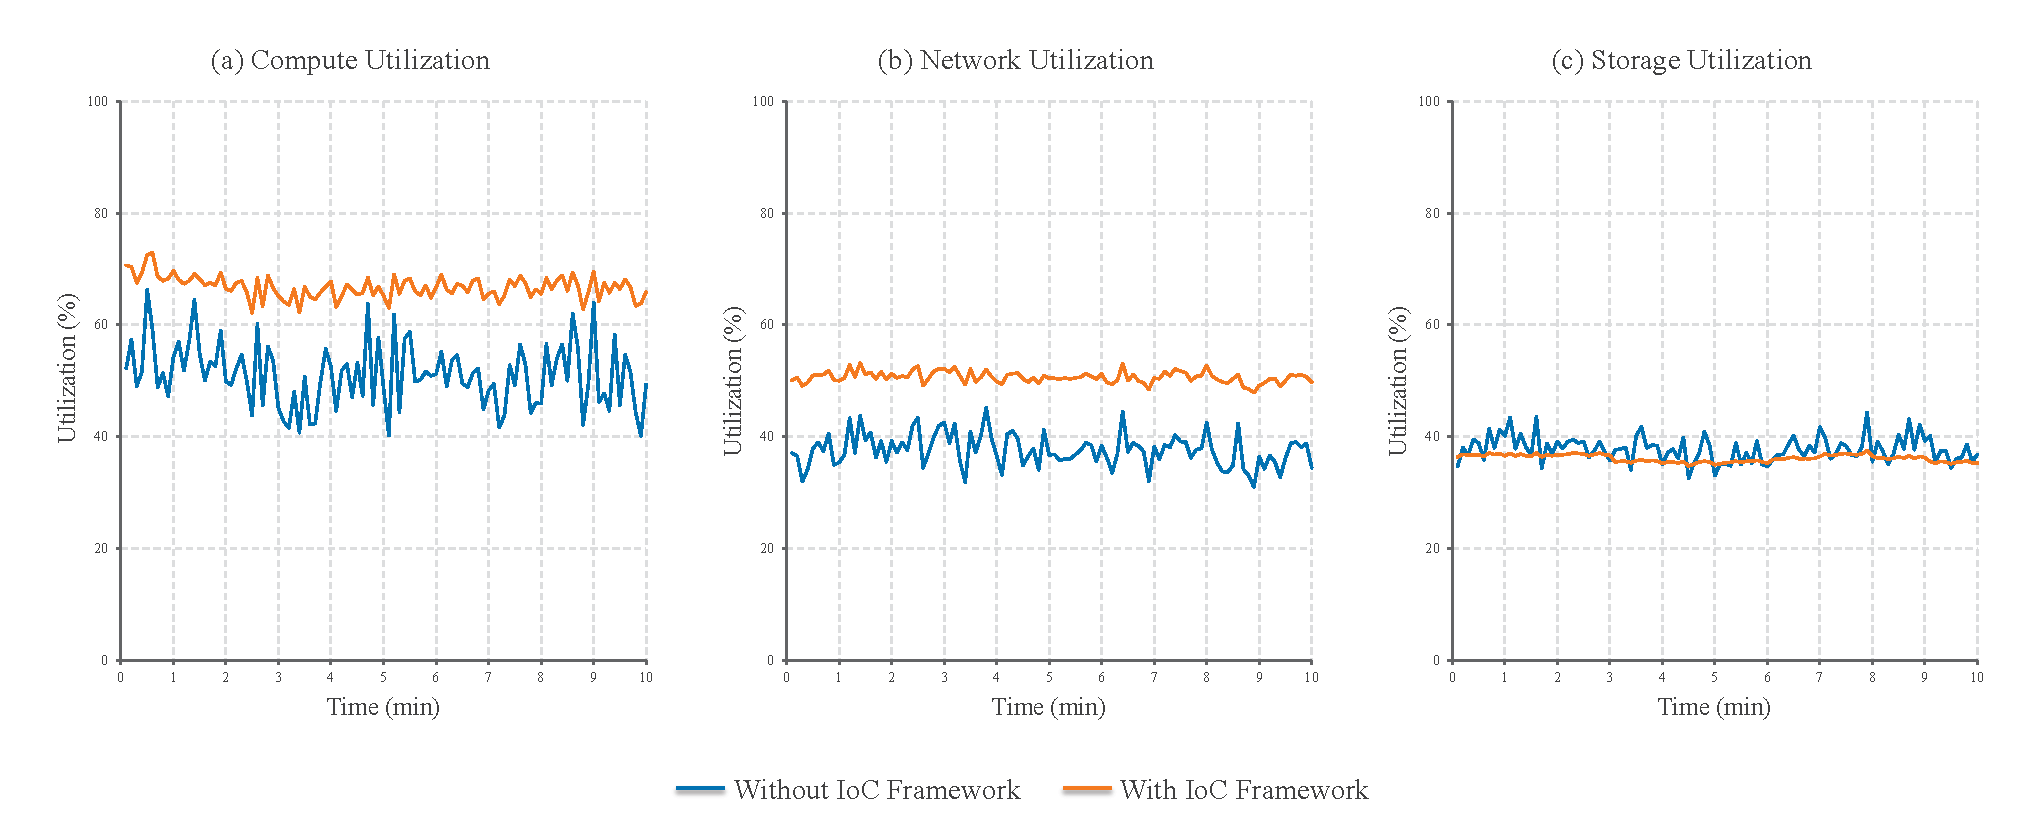
\includegraphics[width=0.90\textwidth]{figures/figure6.1.3-1.eps}
	\caption{Comparison of computing, network, and storage resource utilization.}
	\label{fig:utilization-comparison}
\end{figure*}

\noindent2. Analysis of Resource State Entropy Results

Defining the resource state entropy reduction percentage as $P_i$, we obtain
\begin{equation}
	P_i=1-\frac{H(\mathbf{r}_{I_i})}{H(\mathbf{r}_{t_i})}.
	\label{eq:training-entropy-reduction}
\end{equation}

The comparison of the comprehensive state entropy of the traditional group $H(\mathbf{r}_{t_i})$ and the IoC group $H(\mathbf{r}_{I_i})$ is presented in Table~\ref{tab:weighted-entropy-comparison}.

\begin{table}[!t]
	\centering
	\caption{Analysis of Comprehensive State Entropy Results}
	\label{tab:weighted-entropy-comparison}
	
	\begingroup
	\scriptsize
	\setlength{\tabcolsep}{2.7pt}
	\renewcommand{\arraystretch}{1.05}
	
	\begin{tabular*}{\columnwidth}{
			@{\extracolsep{\fill}}
			cccc
			@{}
		}
		\toprule
		\makecell[c]{\textbf{Time}\\\textbf{(min)}}
		& $H(\mathbf{r}_{t_i})$
		& $H(\mathbf{r}_{I_i})$
		& $P_i$ \\
		\midrule
		1  & 0.433 & 0.197 & 54.4 \\
		2  & 0.465 & 0.183 & 60.7 \\
		3  & 0.435 & 0.225 & 48.2 \\
		4  & 0.434 & 0.212 & 51.1 \\
		5  & 0.42  & 0.189 & 55.1 \\
		6  & 0.387 & 0.211 & 45.6 \\
		7  & 0.411 & 0.189 & 54   \\
		8  & 0.347 & 0.167 & 52   \\
		9  & 0.451 & 0.196 & 56.6 \\
		10 & 0.398 & 0.199 & 50.1 \\
		\midrule
		\multicolumn{3}{c}{Average} & 52.8 \\
		\bottomrule
	\end{tabular*}
	\endgroup
\end{table}

From the perspective of entropy distribution characteristics, all ten observation instants of the IoC group fall within the low-entropy region below 0.3, with no high-entropy outliers; the corresponding values of the traditional group all fall within the medium-to-high entropy range of 0.3--0.5. Overall, the comprehensive state entropy of the IoC group is on average 52.8\% lower than that of the traditional group, and both the entropy level and distribution dispersion are significantly lower than those of the traditional group. Fig.~\ref{fig:entropy-distribution} shows the three-dimensional distribution comparison of the three types of resource state entropy.

This result validates the effectiveness of the entropy balance theory and scheduling algorithm proposed in this paper: it effectively balances load fluctuations, ensures stable node operating states, and resolves the poor system stability caused by the lack of resource-state awareness in traditional architectures.

\begin{figure}[!ht]
	\centering
	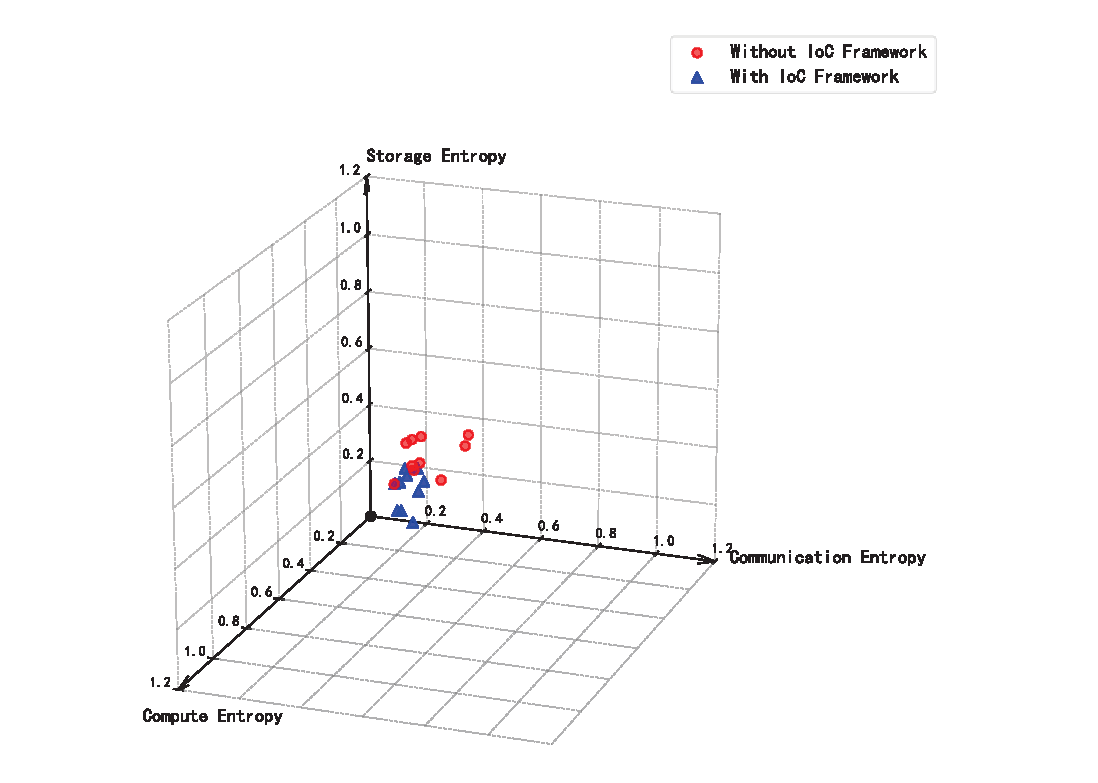
\includegraphics[width=0.90\columnwidth]{figures/figure13.eps}
	\caption{Distribution of resource node state entropy.}
	\label{fig:entropy-distribution}
\end{figure}


\subsection{Experiment on LLM Inference Based on the IoC}
\label{s6-2}

\subsubsection{Experimental Design}
\label{s6-2-1}

\par
\Needspace{3\baselineskip}
\noindent\textit{Experimental Environment Configuration.}\par

The inference model is DeepSeek-R1-0528 (671B), deployed on NVIDIA H20 GPUs (96 GB per GPU), with Experiment 1 and Experiment 2 conducted on the physical deployment platform. 

The experimental environment follows the three-layer architecture of the IoC and comprises the Application Service Layer, Interconnection Resource Layer, and Compute and Network Infrastructure Layer. Computing nodes that meet the requirements of LLM inference are configured to comprehensively evaluate the architecture's optimization performance in inference scenarios.

\par
\Needspace{3\baselineskip}
\noindent\textit{Application Service Layer.}\par

The Application Service Layer is responsible for initiating inference task requests. The performance requirements of inference services are determined based on differences in model scale, computing-resource demand, and response latency among inference tasks. This experiment uses real-time inference calls to the LLM DeepSeek-R1 on the requester side as the core scenario and designs typical inference task loads to provide a controllable benchmark for subsequent node resource scheduling and performance evaluation.

\par
\Needspace{3\baselineskip}
\noindent\textit{Interconnection Resource Layer.}\par

The Interconnection Resource Layer serves as the core layer for implementing the entropy balance theory of the IoC and unified resource orchestration and scheduling through collaboration between the CRID Gateway and the entropy-balanced scheduling algorithm. Based on the five-level positioning and addressing framework Enterprise--City--Computing Center--Server--Chip, the CRID Gateway periodically collects node resource metrics. It then automatically calculates the computing, network, and storage entropy of each node using the resource state entropy formula, providing a quantitative basis for resource state evaluation. The entropy-balanced scheduling algorithm models inference demands using the task parameters $\mu$ and $\lambda$. Inference tasks are characterized by short-term bursts, high-frequency arrivals (high $\lambda$), and short service times (low $\mu$). Using these task characteristics together with the resource state entropy reported by the CRID Gateway, the algorithm dynamically matches inference tasks to nodes with stable states, thereby achieving optimal alignment between task requirements and underlying computing resources.

\par
\Needspace{3\baselineskip}
\noindent\textit{Compute and Network Infrastructure Layer.}\par

The Compute and Network Infrastructure Layer provides the physical computing and transmission resources required to support IoC operation. This experiment constructs an IoC environment comprising heterogeneous computing nodes interconnected through high-speed networks, with differentiated computing, storage, and network capabilities. Each node carries an initial load generated by various computing tasks, such as scientific computing, rendering and live streaming, and inference Q\&A, and the load changes dynamically as these tasks are executed.

\par
\Needspace{3\baselineskip}
\noindent\textit{Experimental Setup.}\par

Progressive experiments are designed along two dimensions: Resource State Stability and task performance. Resource state provides the basis for scheduling decisions, and its fluctuations directly affect the predictability of task execution. Improvements in resource stability should therefore be reflected in task performance gains. Accordingly, the experimental setup includes the following two experiments:

\begin{itemize}[nosep]
	\item Experiment 1: Stability experiment of node resource states under the IoC architecture. This experiment compares the computing entropy, network entropy, and storage entropy of nodes with and without the IoC architecture to verify the architecture's role in improving resource state stability.
	
	\item Experiment 2: Comparative performance experiment between traditional internet architecture and the IoC architecture. Comparison scenarios are established for deployments based on the traditional internet architecture and the IoC architecture to evaluate the actual performance improvements provided by the IoC architecture in inference scenarios.
\end{itemize}

\par
\Needspace{3\baselineskip}
\noindent\textit{Experimental Implementation.}\par

\begin{itemize}[nosep]
\item Experiment 1:
This experiment evaluates the role of the IoC architecture in resource-state awareness and task scheduling for LLM inference. Four GPUs are configured as four independent nodes. Under the same inference workload, the computing, network, and storage resource states of these nodes are compared between conditions with and without the IoC architecture.

Real-time inference with DeepSeek-R1-0528 is used as the primary workload. Requests have fixed input and output lengths of 4k~tokens and 1k~tokens, respectively, with a concurrency level of 64. The four nodes jointly serve the workload in a Prefill/Decode (P/D) disaggregated architecture. Requests are submitted continuously to maintain inference traffic across the four-node system throughout the experiment. Both conditions use the same workload; only the scheduling policy differs, providing a consistent basis for comparison.

Without the IoC architecture, the baseline processes inference requests using a conventional resource-allocation policy. Requests are assigned primarily according to their existing network connections to nodes. As requests continue to arrive, node selection is not coordinated using the real-time resource states of other nodes. Requests may therefore remain concentrated on a small subset of nodes while the others have relatively low resource utilization.

With the IoC architecture, the CRID Gateway continuously monitors the computing, network, and storage resource states of all four nodes. Upon the arrival of a new inference request, the scheduler obtains the nodes' current resource states, calculates the corresponding resource-state entropy values, and selects an execution node based on the task requirements and node states. Subsequent requests are matched again when node resource states change.

\item Experiment 2: A unified task load and model structure are used across different configurations to ensure comparability. Data are collected and analyzed over multiple rounds under high-concurrency conditions. Task loads are generated following standard benchmarking methods used by open-source LLM inference frameworks, with two typical workload-generation methods:

\begin{itemize}[nosep]
	\item Fixed concurrency stress test: To represent resource-intensive and computing-intensive workloads, the maximum number of simultaneously active inference requests is limited, and the concurrency level is gradually increased in integer steps to evaluate the system's resource scheduling boundaries and stability.
	
	\item Dynamic request rate test: This test simulates the inference-request load characteristics of small- and medium-sized LLMs in high-concurrency scenarios. A Poisson distribution is used to simulate user request flows, with request rates increased stepwise to detect throughput limits and response latency variations.
\end{itemize}

\end{itemize}
To ensure the statistical representativeness of the experimental data and the adequacy of the comparative analysis, each test includes at least 1000 requests.

\subsubsection{Experimental Procedure}
\label{s6-2-2}

\par
\Needspace{3\baselineskip}
\noindent\textit{Experiment 1: Stability Experiment of Node Resource States under the IoC Architecture.}\par

The four GPUs are deployed as four independent nodes in a P/D disaggregated architecture. Node~1 serves as the D node, whereas Nodes~2,~3, and~4 serve as P nodes. Resource states are collected from all four nodes, with subsequent measurements and analysis focusing primarily on the three Prefill nodes to characterize changes in their computing, network, and storage states.

The CRID Gateway periodically collects the following resource metrics from all four nodes:
\begin{itemize}[nosep]
	\item Computing resources: GPU utilization is measured as the proportion of the observation interval during which the GPU is actively working. It directly represents computing-resource utilization.
	
	\item Network resources: Network throughput is measured for each node. Bandwidth utilization is calculated as the ratio of observed throughput to the bandwidth available to that node and represents its network-resource usage.
	
	\item Storage resources: Storage-space usage is measured for each node. Storage occupancy is calculated as the ratio of used storage space to the node's usable storage capacity and represents its storage-resource usage.
\end{itemize}

The observation period is 24~h, divided into 1-h statistical intervals. Resource utilization is sampled throughout each interval and summarized as one hourly mean and its corresponding resource state. This yields 24 observations per node for each resource type. The collected data are used to calculate the computing, network, and storage entropy of all four nodes.

The evaluation metrics are defined as follows:
\begin{itemize}[nosep]
	\item Computing entropy: calculated from the probability distribution of GPU utilization across the utilization intervals over the 24-h observation period, using the computing-resource state entropy equation in Section~\ref{s3-4}.
	
	\item Network entropy: calculated from the probability distribution of bandwidth utilization across the same intervals, using the network-resource state entropy equation in Section~\ref{s3-4}.
	
	\item Storage entropy: calculated from the probability distribution of storage occupancy across the same intervals, using the storage-resource state entropy equation in Section~\ref{s3-4}.
\end{itemize}

All three resource types use the four state intervals defined in Section~\ref{s3-4-1}: $[0,30\%]$, $[30\%,60\%]$, $[60\%,80\%]$, and $[80\%,100\%]$. For each node and resource type, the number of hourly observations falling into each interval is divided by the total of 24 observations to obtain the corresponding state probability. These probabilities are then substituted into the relevant entropy equation.

The inference workload is first run without the IoC architecture. Requests are assigned according to the baseline policy, and resource states are collected throughout the observation period. All four nodes are then reset to the same initial resource states as in the baseline run. The experiment is repeated with the IoC architecture while the model, inference requests, and workload are held constant.

After both runs, the distributions of resource utilization across the four intervals are determined for each node. Computing, network, and storage entropy are then calculated for all four nodes under each architecture to obtain the comparative results.

\par
\Needspace{3\baselineskip}
\noindent\textit{Experiment 2: Comparative Performance Experiment between Traditional Internet Architecture and the IoC Architecture.}\par

This experiment focuses on verifying the impact of the IoC architecture on distributed-node inference relative to the traditional Internet architecture in terms of processing mode, network capacity, and physical distance. Three controlled groups are configured with equivalent computing resources.

\begin{itemize}[nosep]
	\item Group 1: Random centralized nodes in the traditional Internet architecture. This group adopts the traditional protocol stack without the Interconnection Resource Layer. All inference tasks are processed serially on the same computing node. The group has no CRID awareness or dynamic scheduling capability and serves as the baseline for traditional centralized inference.
	
	\item Group 2: Random distributed nodes in the traditional Internet architecture. This group adopts the traditional protocol stack without the Interconnection Resource Layer. Inference tasks are scheduled to multiple geographically distributed nodes for parallel processing. Inter-node network bandwidth is limited to simulate public network transmission. The group has no node resource state entropy perception or entropy-balanced scheduling mechanism.
	
	\item Group 3: Random distributed nodes in the IoC architecture. This group fully deploys the three-tier architecture IoC architecture. The CRID Gateway perceives the computing entropy, network entropy, and storage entropy of each node in real time. The entropy-balanced scheduling algorithm dynamically matches inference tasks to nodes with the lowest comprehensive state entropy, thereby enabling cross-domain distributed parallel inference. This group evaluates the comprehensive performance advantages of the IoC architecture in distributed mode.
\end{itemize}

The evaluation metrics selected are TTFT (Time to First Token), defined as the latency from request submission to the generation of the first output token, and TPOT (Time Per Output Token), defined as the average interval between adjacent output tokens. Accordingly, Time To First Token (TTFT) and Time Per Output Token (TPOT) are selected as dependent variables to characterize the qualitative relationship between transmission time and inference latency. To examine how different input-output lengths affect this relationship, three input-output length configurations are used: 1024--1024 tokens, 2048--2048 tokens, and 4096--4096 tokens.

The three comparison groups use the same model, inference configuration, workload, and total computing-resource budget, while their processing mode, network conditions, and scheduling mechanisms are varied according to the experimental design.

Before calculating TTFT and TPOT, failed, timed-out, or incomplete requests are excluded as invalid measurements. For each architecture group, input-output length, concurrency level, and metric, statistical outliers are then identified using the Tukey 1.5$\times$IQR rule, where observations below $Q_1$-1.5IQR or above $Q_3$+1.5IQR are excluded. The same procedure is applied independently to TTFT and TPOT for all comparison groups.

\subsubsection{Experimental Results}
\label{s6-2-3}

\par
\Needspace{3\baselineskip}
\noindent\textit{Experiment 1: Stability Experiment of Node Resource States under the IoC Architecture.}\par

Based on the 24 hourly observations, we counted how often each node occupied each of the four resource-state intervals and calculated the corresponding state entropy. Tables~\ref{tab:inference-state-baseline} and~\ref{tab:inference-state-ioc} report the results without and with the IoC architecture, respectively.

\begin{table*}[!t]
	\centering
	\caption{Resource-state interval counts and entropy without the IoC architecture.}
	\label{tab:inference-state-baseline}
	\scriptsize
	\setlength{\tabcolsep}{5pt}
	\renewcommand{\arraystretch}{1.08}
	\begin{tabular*}{\textwidth}{@{\extracolsep{\fill}}llccccc@{}}
		\toprule
		\textbf{Node} & \textbf{Resource}
		& \textbf{$[0,30\%]$}
		& \textbf{$[30\%,60\%]$}
		& \textbf{$[60\%,80\%]$}
		& \textbf{$[80\%,100\%]$}
		& \makecell[c]{\textbf{State entropy}\\\textbf{(bits)}} \\
		\midrule
		\multirow{3}{*}{Node~1}
		& Computing & 0 & 2  & 16 & 6 & 1.189 \\
		& Network   & 0 & 5  & 16 & 3 & 1.236 \\
		& Storage   & 0 & 22 & 2  & 0 & 0.414 \\
		\midrule
		\multirow{3}{*}{Node~2}
		& Computing & 0 & 3  & 17 & 4 & 1.158 \\
		& Network   & 0 & 6  & 15 & 3 & 1.299 \\
		& Storage   & 0 & 21 & 3  & 0 & 0.544 \\
		\midrule
		\multirow{3}{*}{Node~3}
		& Computing & 2 & 10 & 9  & 3 & 1.731 \\
		& Network   & 3 & 13 & 8  & 0 & 1.382 \\
		& Storage   & 0 & 10 & 14 & 0 & 0.980 \\
		\midrule
		\multirow{3}{*}{Node~4}
		& Computing & 24 & 0 & 0 & 0 & 0.000 \\
		& Network   & 24 & 0 & 0 & 0 & 0.000 \\
		& Storage   & 24 & 0 & 0 & 0 & 0.000 \\
		\bottomrule
	\end{tabular*}
\end{table*}

\begin{table*}[!t]
	\centering
	\caption{Resource-state interval counts and entropy with the IoC architecture.}
	\label{tab:inference-state-ioc}
	\scriptsize
	\setlength{\tabcolsep}{5pt}
	\renewcommand{\arraystretch}{1.08}
	\begin{tabular*}{\textwidth}{@{\extracolsep{\fill}}llccccc@{}}
		\toprule
		\textbf{Node} & \textbf{Resource}
		& \textbf{$[0,30\%]$}
		& \textbf{$[30\%,60\%]$}
		& \textbf{$[60\%,80\%]$}
		& \textbf{$[80\%,100\%]$}
		& \makecell[c]{\textbf{State entropy}\\\textbf{(bits)}} \\
		\midrule
		\multirow{3}{*}{Node~1}
		& Computing & 0 & 3  & 16 & 5 & 1.236 \\
		& Network   & 0 & 10 & 12 & 2 & 1.325 \\
		& Storage   & 3 & 20 & 1  & 0 & 0.785 \\
		\midrule
		\multirow{3}{*}{Node~2}
		& Computing & 0 & 4  & 15 & 5 & 1.326 \\
		& Network   & 0 & 11 & 10 & 3 & 1.417 \\
		& Storage   & 2 & 19 & 3  & 0 & 0.941 \\
		\midrule
		\multirow{3}{*}{Node~3}
		& Computing & 1 & 6  & 14 & 3 & 1.520 \\
		& Network   & 1 & 9  & 12 & 2 & 1.520 \\
		& Storage   & 3 & 18 & 3  & 0 & 1.061 \\
		\midrule
		\multirow{3}{*}{Node~4}
		& Computing & 1 & 7  & 13 & 3 & 1.564 \\
		& Network   & 1 & 10 & 11 & 2 & 1.532 \\
		& Storage   & 4 & 18 & 2  & 0 & 1.041 \\
		\bottomrule
	\end{tabular*}
\end{table*}

Without the IoC architecture, resource-state distributions differ substantially across nodes. Nodes~1 and~2 spend most computing observations in the $[60\%,80\%]$ or $[80\%,100\%]$ intervals, whereas all 24 computing, network, and storage observations for Node~4 fall in the $[0,30\%]$ interval. This pattern indicates uneven resource use across the nodes.

With the IoC architecture, computing utilization for all four nodes occurs predominantly in the $[60\%,80\%]$ interval. Network utilization is distributed mainly across the $[30\%,60\%]$ and $[60\%,80\%]$ intervals, while storage occupancy occurs predominantly in the $[30\%,60\%]$ interval. The resource-state distributions are more similar across nodes than under the baseline condition, consistent with reduced concentration of requests on a small subset of nodes.

Under the same real-time inference workload, state-aware scheduling redistributes requests as node conditions change, shifting resource use from a strongly uneven pattern toward a more similar distribution across the four nodes. Jointly considering computing, network, and storage states thus reduces between-node differences in resource use and supports cross-node resource coordination for real-time LLM inference.

\par
\Needspace{3\baselineskip}
\noindent\textit{Experiment 2: Comparative Performance Experiment between Traditional Internet Architecture and the IoC Architecture.}\par

As shown in Figure~\ref{fig:Performance of TTFT and TPOT under different scenarios}, the experimental results reveal a clear performance gradient among the three groups in terms of TTFT and TPOT. Group 3, which uses the IoC architecture, performs best, followed by the random distributed-node group under the traditional Internet architecture, whereas the random centralized-node group performs worst.

\begin{figure*}[!t]
	\centering
	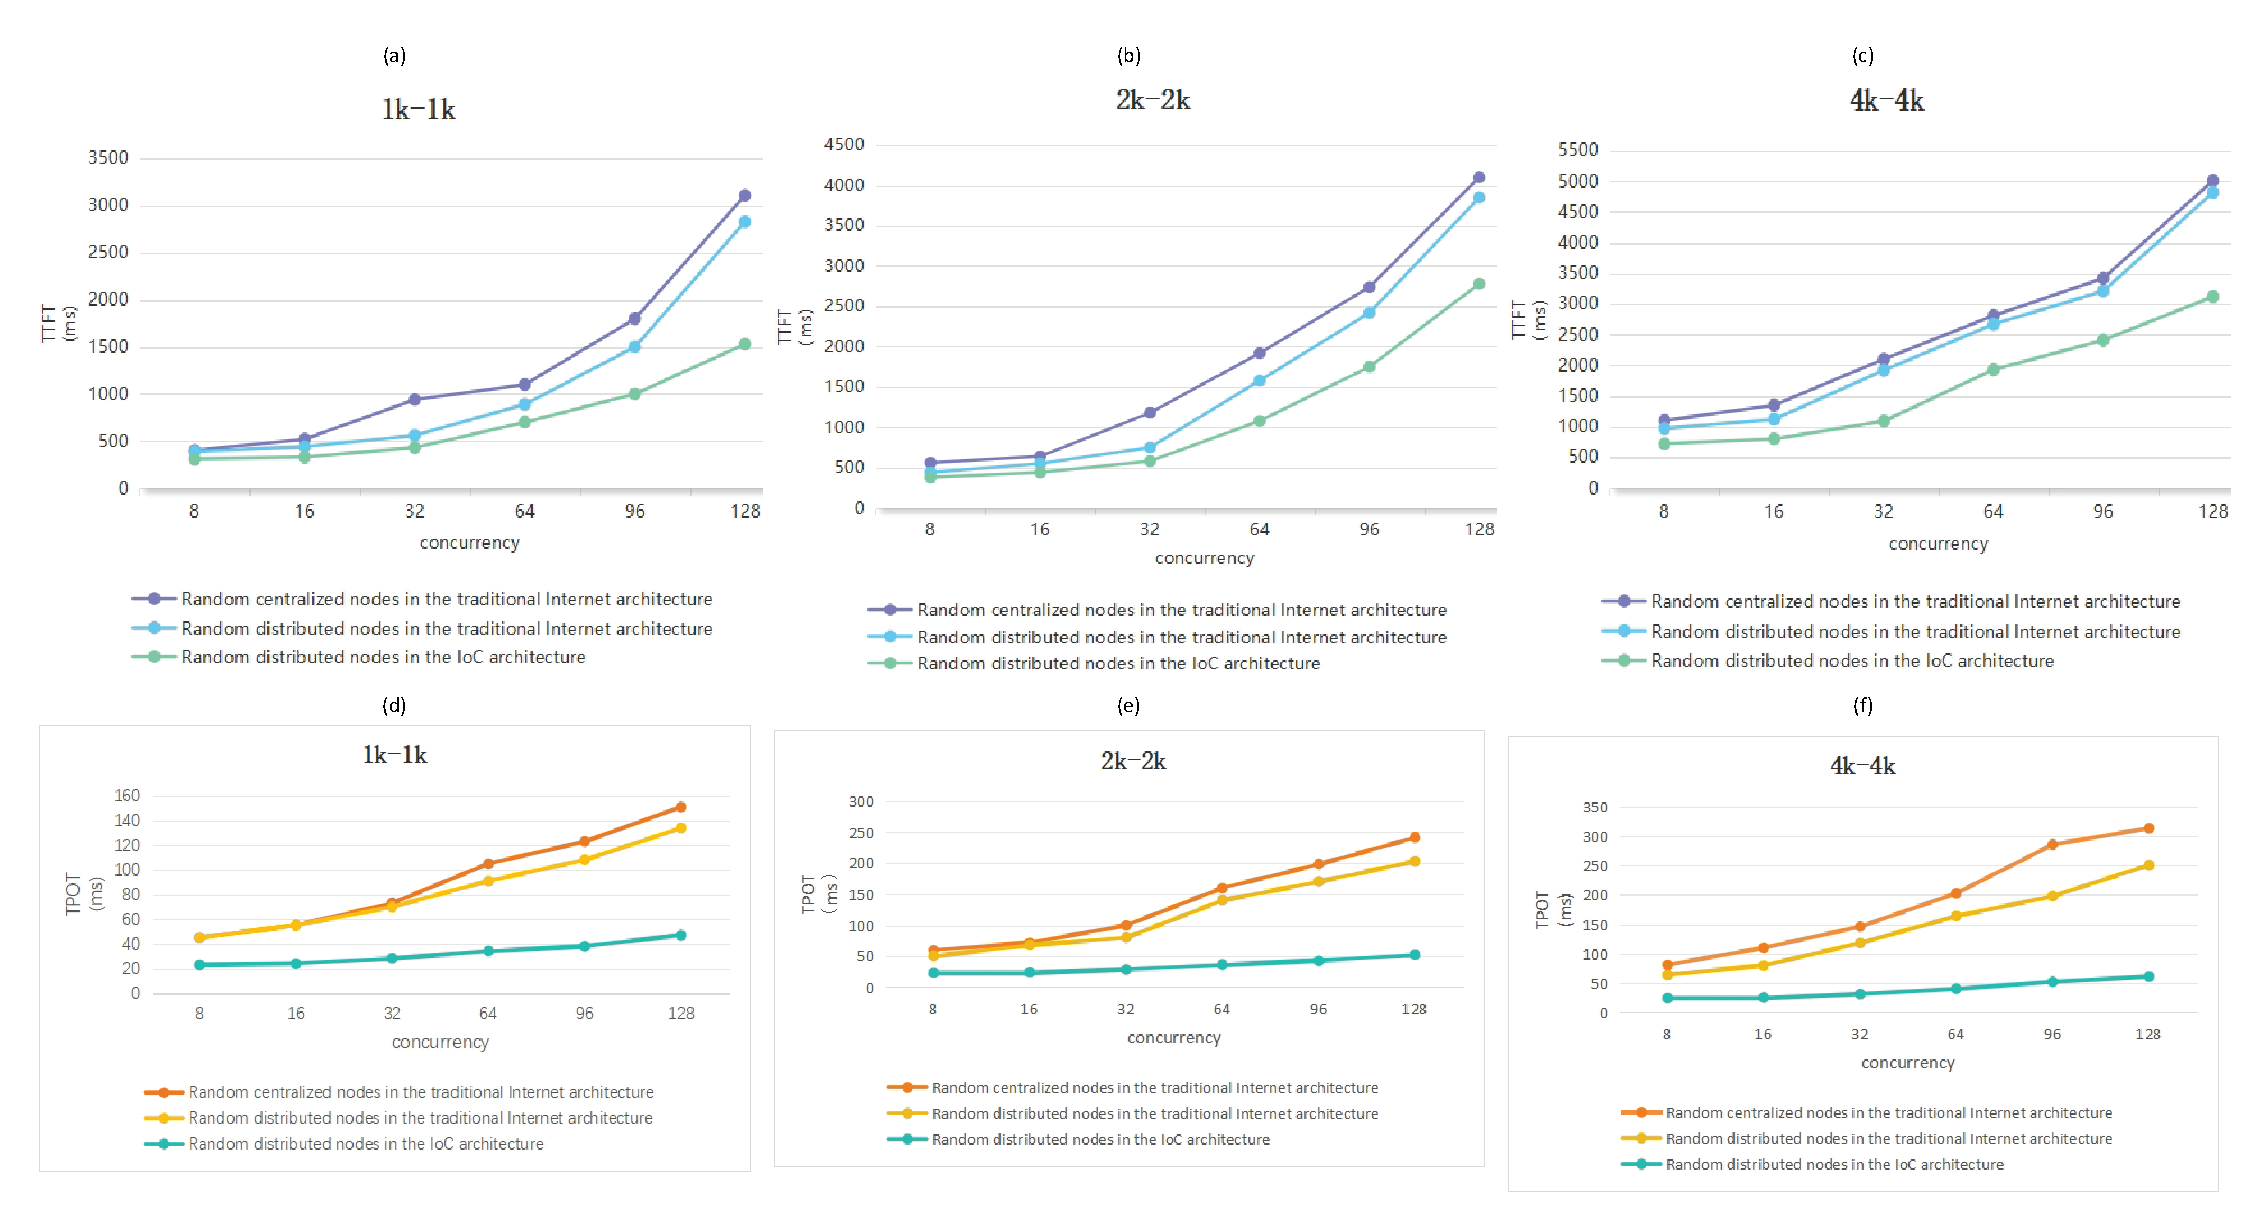
\includegraphics[width=0.96\textwidth]{figures/figure15.eps}
	\caption{Performance of TTFT and TPOT under different scenarios.}
	\label{fig:Performance of TTFT and TPOT under different scenarios}
\end{figure*}

This ranking demonstrates that under the same deployment mode, the IoC architecture significantly outperforms the traditional Internet architecture. Under the same architecture, random distributed inference outperforms random centralized inference. Overall, the optimal performance achieved under the IoC architecture verifies the comprehensive advantages of computing and network convergence and entropy-balanced scheduling.

\par
\Needspace{3\baselineskip}
\noindent 1) \textit{Formation Mechanism of Performance Differences.}\par

\begin{itemize}[nosep]
	\item Group 1 (Random centralized nodes in the traditional Internet architecture): This group is limited by the computing-resource ceiling of a single node and lacks the capability to perceive node states through the CRID Gateway. As the number of concurrent requests increases, the queuing delay increases rapidly as the number of concurrent requests grows, leading to rapid deterioration in TTFT. As the baseline control, this group reflects the performance boundary of random centralized inference in the traditional Internet architecture under the most unfavorable conditions.
	
	\item Group 2 (Random distributed nodes in the traditional Internet architecture): Although this group adopts random distributed parallel processing, it has limited inter-node network bandwidth and lacks resource state entropy perception and entropy-balanced scheduling. As described in Chapter 3, inference tasks are characterized by high $\lambda$ (high-frequency arrivals) and low $\mu$ (short service time). In the traditional distributed architecture, limited network bandwidth and the lack of resource-state-aware scheduling can lead to communication bottlenecks and imbalanced node workloads, causing Group 2 to exhibit significantly worse TPOT than Group 3 in long-context scenarios. This result demonstrates how the Compute and Network decoupling limits the performance of distributed inference under the traditional Internet architecture.
	
	\item Group 3 (Random distributed nodes in the IoC architecture): This group constructs a global resource view through the CRID Gateway. The entropy-balanced scheduling algorithm dynamically allocates inference tasks to multiple low-entropy nodes for parallel processing and supports cross-domain high-speed data transmission. As described in Section 4.3, the control-plane separation design of the Interconnection Resource Layer enables the system to optimize both computing parallelism and network efficiency. Its optimal performance across all test scenarios verifies the synergistic gain of random distributed parallelism and Compute and Network convergence.
\end{itemize}

\par
\Needspace{3\baselineskip}
\noindent 2) \textit{Further Analysis in Long-Context and High-Concurrency Scenarios.}\par

Across tests with different context lengths, longer contexts further amplify the architectural differences. When the input-output length increases to 4096--4096 tokens, the gap in TPOT between Group 2 and Group 3 widens significantly.

The demand for network bandwidth grows linearly with long-sequence transmission. The traditional Internet architecture lacks the ability to perceive and schedule network state entropy. Consequently, the cumulative effect of transmission delay caused by bandwidth constraints becomes more pronounced, increasing the proportion of communication time in Group 2 from 15\% in short-context scenarios to approximately 35\% in long-context scenarios. In contrast, Group 3 monitors network resource state entropy in real time through the CRID Gateway and preferentially assigns long-context tasks to low-entropy nodes, effectively limiting the increase in the proportion of communication time.

For the 1k–1k contexting scenario, as concurrency increases from 8 to 128, TTFT rises from 310 to 1530 ms for Group 3 and from 390 to 2830 ms for Group 2. At 128 concurrency, Group 3’s TTFT is $54.1\%$ of Group 2’s. This is because the IoC architecture distributes bursty requests across multiple low-entropy nodes through the entropy-balanced scheduling algorithm, avoiding the exponential growth of queuing latency caused by single-node overload in traditional architectures.

\section{Conclusion}
\label{s7}
In summary, the IoC architecture theoretically solves the inherent defects of traditional architectures in heterogeneous resource scheduling, network state perception, and precise task matching through quantitative perception of resource state entropy, dynamic entropy-balanced scheduling, and deep Compute and Network collaboration. The superior experimental performance empirically demonstrates the effectiveness of IoC in real heterogeneous computing environments, laying solid architectural foundations for building large-scale, high-concurrency, low-latency services over the computing internet.

\flushbottom
\bibliography{myref}

\biographies

\begin{CCJNLbiography}{figures/author/WeiLi.eps}{Li Wei}
	is a professor of engineering. She currently works at the China Academy of Information and Communications Technology (CAICT), Beijing, China, where she has been engaged in research on cloud computing, artificial intelligence, making significant contributions to the establishment of internet of compute (IoC) architecture. She has published more than ten academic papers and holds more than 20 invention patents. Email: liwei3@caict.ac.cn
\end{CCJNLbiography}

\begin{CCJNLbiography}{figures/author/WeiboZhao.eps}{Zhao Weibo}
	graduated from Beijing University of Posts and Telecommunications, Beijing, China, with a master’s degree. He is currently a cloud computing researcher and engineer at the China Academy of Information and Communications Technology (CAICT), Beijing, China. His main research interests include cloud computing, high-performance networking, and cloud-network integration. He has published more than ten SCI/EI academic papers. Email: zhaoweibo@caict.ac.cn
\end{CCJNLbiography}

\begin{CCJNLbiography}{figures/author/RunyanWang.eps}{Wang Runyan}
	received his M.S. degree from China Academy of Telecommunication Technology, Beijing, China, in 2024. He is currently an engineer at the China Academy of Information and Communications Technology (CAICT), Beijing, China. His research fields include computing power network, computing power identification, and cloud operating systems. He has published 5 papers in core journals, 4 software copyrights, and 1 invention patent. Email: wangrunyan@caict.ac.cn
\end{CCJNLbiography}

\begin{CCJNLbiography}{figures/author/LiuSang.eps}{Sang Liu}
	graduated from Xidian University, Xi'an, China, with a master's degree and currently works at the China Academy of Information and Communications Technology (CAICT), Beijing, China, as an engineer. Her main research areas are cloud computing, high-performance networks, and internet of compute, and she has published several EI-indexed papers. Email: sangliu@caict.ac.cn
\end{CCJNLbiography}

\begin{CCJNLbiography}{figures/author/JinfeiHuang.eps}{Huang Jinfei}
	graduated from City University of Hong Kong, Hong Kong, China, with a master's degree. He is currently an intermediate engineer at the China Academy of Information and Communications Technology (CAICT), Beijing, China. His main research interests include artificial intelligence and cloud computing. His major academic achievements include publishing the paper “Task and Resource Collaborative Orchestration and Scheduling Algorithm Based on Computing Resource Interconnected Network” at an international conference. Email: huangjinfei@caict.ac.cn
\end{CCJNLbiography}

\begin{CCJNLbiography}{figures/author/SonglinSun.eps}{Sun Songlin}
	, Ph.D., is a professor at Beijing University of Posts and Telecommunications, Beijing, China. His main research areas are wireless communication, multimedia technology, and artificial intelligence. Email: slsun@bupt.edu.cn
\end{CCJNLbiography}

\begin{CCJNLbiography}{figures/author/RumingLiu.eps}{Liu Ruming}
	is an engineer at the China Academy of Information and Communications Technology (CAICT), Beijing, China. He is responsible for advancing initiatives in internet of compute and cloud-native artificial intelligence. Email: liuruming@caict.ac.cn
\end{CCJNLbiography}

\begin{CCJNLbiography}{figures/author/YueSu.eps}{Su Yue}
	is a senior engineer at the China Academy of Information and Communications Technology (CAICT), Beijing, China. He holds a master's degree in engineering from Beijing University of Posts and Telecommunications, Beijing, China. His current research focuses on artificial intelligence, cloud computing, computing power, cloud networks, internet of compute, and high-performance networks. He has published numerous SCI and EI papers. Email: suyue1@caict.ac.cn
\end{CCJNLbiography}

\begin{CCJNLbiography}{figures/author/FeiMa.eps}{Ma Fei}
	is a senior engineer and holds a Ph.D. from Beijing Jiaotong University, Beijing, China, and currently works at the China Academy of Information and Communications Technology (CAICT), Beijing, China. His main research areas are cloud computing, artificial intelligence, internet of compute, and high-performance networks. He has published numerous EI papers. Email: mafei@caict.ac.cn
\end{CCJNLbiography}

\end{document}
